% slide di panoramica sulla tecnologia XML
% % Panoramica XML: definizione, sintassi, documento ben formato, documento valido
% cos'è XML
% XML is used when you want to mark up a textual resource and to store data in a suitable and recognized standard way.

%% slide premesse


\documentclass{beamer}
    
    %    \usepackage[english]{babel}
        %\usepackage[latin1]{inputenc}
        %\usepackage[T1]{fontenc}
    
    \mode<presentation>{
      \setbeamertemplate{background canvas}[vertical shading]
      \usetheme{Berkeley}
      \useoutertheme{himinfolines}
    }
      
    \usepackage{ucs}
    \usepackage[utf8]{inputenc}
    \usepackage[english,polutonikogreek,italian,UKenglish,british]{babel}
    \usepackage{graphicx}
    \usepackage{colortbl}
    \usepackage{multicol}
    \usepackage{ulem}
    \usepackage{verbatim}
    \usepackage{alltt}
    \usepackage{ccicons}
    \usepackage{MnSymbol,wasysym}
    \usepackage{tikzsymbols}
    \usepackage{textcomp}
    \usepackage{xmpincl}
    
    \usepackage{parskip}
    \setcounter{nframes}{100}
    \setcounter{nframe}{1}
    \setbeamercovered{dynamic}
    \newenvironment{grcenv}{\begin{otherlanguage}{greek}}{\end{otherlanguage}}
    \newcommand{\g}[1]{\textgreek{#1}}
    \definecolor{darkgreen}{rgb}{0,0.5,0}
    \definecolor{darkblue}{rgb}{0,0,0.5}
    \definecolor{grey}{rgb}{0.5,0.5,0.5}
    \setcounter{tocdepth}{5}
    
    \makeatletter
    
    \makeatother
    %\includexmp{LicencesAndLicensing}
    
    %frame00 metadata
        \title{Codifica di Testi - Introduzione XML Markup \\a.a. 2018-2019}
        \author[A.M. Del Grosso]{Angelo Mario Del Grosso}
        \institute{\texttt{angelo.delgrosso@ilc.cnr.it} \\\bigskip\textit{CNR-ILC-LicoLab}}
        \date{Istituto di Linguistica Computazionale ``A. Zampolli'', \today}
        \AtBeginSection[]{
        \begin{frame}<beamer>
        \addtocounter{nframe}{1}
        \footnotesize
        \frametitle{Progress status}
        \tableofcontents[currentsection,hideothersubsections]
        \end{frame}
        }
    
\begin{document}

\begin{frame}
	\maketitle
\end{frame}

\begin{frame}
	\frametitle{Contenuto della lezione}
	\tableofcontents
\end{frame}

\section{I linguaggi di codifica}
\begin{frame}
	\frametitle{I linguaggi di codifica}
	\framesubtitle{introduzione}
	\addtocounter{nframe}{1}

	\begin{block}{Definizione di codifica digitale del testo}
		Per \textbf{codifica} digitale dei testi intendiamo la \textit{rappresentazione formale} di un \textbf{testo} ad un qualche livello descrittivo, su di un supporto digitale, in un formato utilizzabile da un elaboratore (\textit{Machine Readable Form}) mediante un opportuno \textbf{linguaggio informatico} (F. Ciotti).
	\end{block}

\end{frame}

\begin{frame}
	\frametitle{I linguaggi di codifica}
	\framesubtitle{Riassumendo}
	\addtocounter{nframe}{1}

	\begin{block}{Impostazione teorico-pratica}

		\begin{itemize}
			\item  un testo è molto di più della sequenza di caratteri che lo
			      compongono
			\item per mezzo della codifica vogliamo rendere esplicite le
			      caratteristiche che vogliamo analizzare
			\item  solo quello che è esplicito può essere interpretato ed
			      elaborato dal computer
			\item vogliamo codificare il testo per quello che è, non per quello che
			      sembra
			\item codifica da effettuare mediante linguaggio di markup
		\end{itemize}

	\end{block}

\end{frame}


\begin{frame}
	\frametitle{I linguaggi di codifica}
	\framesubtitle{Linguaggi di marcatura}
	\addtocounter{nframe}{1}

	\begin{block}{Il markup}
		Il termine markup è stato utilizzato in passato per denotare i segni grafici che accompagnavano un testo apposti sul documento per indicare correzioni o modalità grafiche di stampa.
	\end{block}

\end{frame}

\begin{frame}
	\frametitle{I linguaggi di codifica}
	\framesubtitle{Linguaggi di marcatura}
	\addtocounter{nframe}{1}

	\begin{center}
		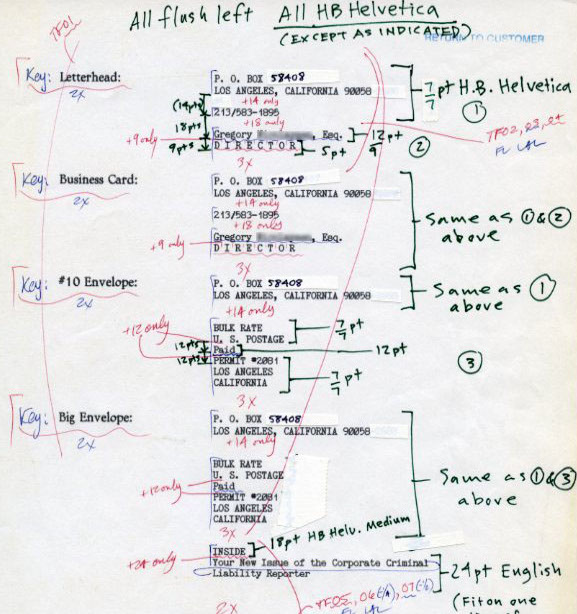
\includegraphics[width=.7\textwidth]{imgs/markup001.jpg}
	\end{center}

\end{frame}

\begin{frame}
	\frametitle{I linguaggi di codifica}
	\framesubtitle{Linguaggi di marcatura}
	\addtocounter{nframe}{1}

	\begin{center}
		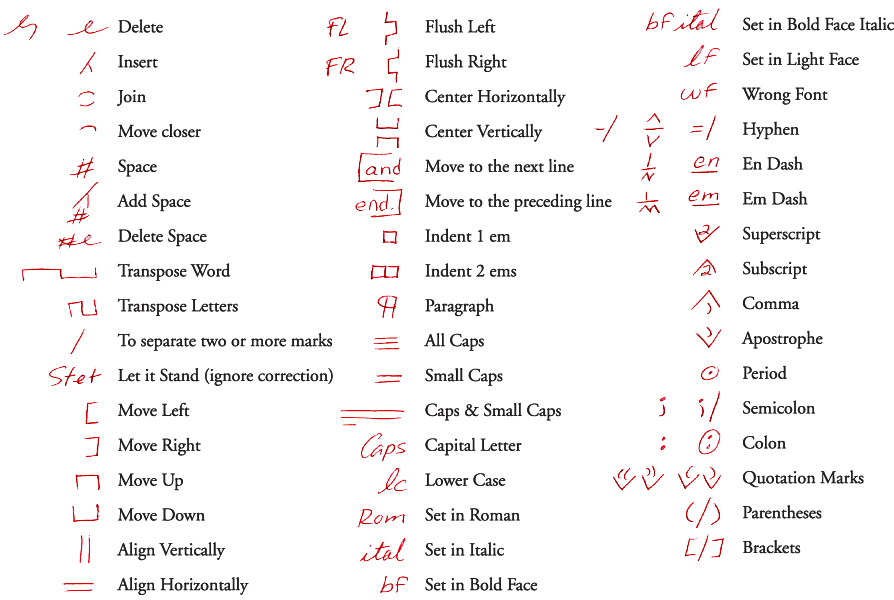
\includegraphics[width=.8\textwidth]{imgs/MarkupConvention.png}
	\end{center}

\end{frame}

\begin{frame}
	\frametitle{I linguaggi di codifica}
	\framesubtitle{Linguaggi di marcatura}
	\addtocounter{nframe}{1}

	\begin{block}{Il markup}
		La codifica con linguaggi di marcatura (markup) è in definitiva un insieme di convenzioni, rese attraverso specifiche sequenze di caratteri, etichette, codici, (detti tags) intercalati nel testo per permettere agli elaboratori elettronici di distinguere le varie parti di un documento.
	\end{block}

	\begin{block}{Il markup formale}
		Un linguaggio di markup è un sistema formale per scambiare e pubblicare informazioni in formato testo in modo strutturato.
	\end{block}


\end{frame}

\begin{frame}
	\frametitle{I linguaggi di codifica}
	\framesubtitle{Linguaggi di marcatura}
	\addtocounter{nframe}{1}

	\begin{block}{Il markup formale}
		Markup formale: costituito da un sistema ben preciso di istruzioni, ognuna delle quali è dotata di una specifica semantica e sintassi.
	\end{block}


\end{frame}

\begin{frame}
	\frametitle{I linguaggi di codifica}
	\framesubtitle{Linguaggi di marcatura}
	\addtocounter{nframe}{1}

	\begin{block}{Diversi tipi di markup}
		Esistono diversi linguaggi di markup, per rappresentare diversi tipi di documenti.
		\begin{itemize}
			\item Linguaggi procedurali (specific markup languages)
			\item Linguaggi dichiarativi (generic markup languages)
		\end{itemize}
	\end{block}
\end{frame}

\begin{frame}
	\frametitle{I linguaggi di codifica}
	\framesubtitle{Linguaggi di marcatura procedurale}
	\addtocounter{nframe}{1}

	\begin{block}{Linguaggi procedurali}
		\begin{itemize}
			\item Orientati al documento, indicano come deve essere elaborato e
			      disposto il testo
			\item Istruzioni da inserire nel testo per specificarne specifiche
			      caratteristiche
			\item Font, dimensione, spaziatura del carattere, posizionamento
			      nella pagina, colore, etc.
		\end{itemize}
	\end{block}

	\textit{Esempi: TeX e LaTeX, RTF}

\end{frame}

\begin{frame}[fragile]
	\frametitle{I linguaggi di codifica}
	\framesubtitle{Linguaggi di marcatura procedurale}
	\addtocounter{nframe}{1}

	\defverbatim{\rtf}{%
		\begin{tiny}
			\begin{verbatim}

    {\rtf1\ansi\deff0\adeflang1025
    {\fonttbl{\f0\froman\fprq2\fcharset0 Times New Roman;}
    {\f1\froman\fprq2\fcharset0 Times New Roman;}
    {\f2\fnil\fprq2\fcharset0 Lucida Sans Unicode;}
    {\colortbl;\red0\green0\blue0;\red128\green128\blue128;}
    {\stylesheet{\s1\cf0{\*\hyphen2\hyphlead2\hyphtrail2\hyphmax0}
    \rtlch\af5\afs24\lang255\ltrch\dbch\af2\afs24\langfe255
    \loch\f0\fs24\lang1040\snext1 Standard;}

        \end{verbatim}
		\end{tiny}
	}

	\begin{block}{Esempio RTF}
		{\rtf}
	\end{block}

\end{frame}

\begin{frame}
	\frametitle{I linguaggi di codifica}
	\framesubtitle{Linguaggi di marcatura procedurale}
	\addtocounter{nframe}{1}

	\begin{block}{Esempio LaTex}
		\begin{tiny}
			Ciao
			%\backslash documentclass$\[a4paper,10pt\]$$\{article\}$\\
			% \backslash usepackage[utf8]$\{inputenc\}$\\
			% \backslash usepackage[T1]$\{fontenc\}$\\
			% \backslash usepackage[italian]$\{babel\}$\\
			% \backslash title$\{Il mio primo documento\}$\\
			% \backslash author$\{Angelo Mario Del Grosso\}$\\
			% \backslash begin$\{document\}$\\
			% \backslash maketitle\\
			% \backslash begin$\{abstract\}$\\
			% Primo tentativo di scrivere in \backslash LaTeX .\\
			% \backslash end$\{abstract\}$\\
			% \backslash section$\{titolo della sezione\}$\\
			% Questo documento è vuoto.\\
			% \backslash footnote$\{nota a piè di pagina.\}$\\
			% \backslash end$\{document\}$\\
		\end{tiny}
	\end{block}

\end{frame}

\begin{frame}
	\frametitle{I linguaggi di codifica}
	\framesubtitle{Linguaggi di marcatura}
	\addtocounter{nframe}{1}

	\begin{block}{Il markup procedurale}
		L’unico utilizzo di un testo codificato tramite un linguaggio procedurale è la creazione di un output orientato alla visualizzazione.
	\end{block}
\end{frame}

\begin{frame}
	\frametitle{I linguaggi di codifica}
	\framesubtitle{Linguaggi di marcatura procedurale}
	\addtocounter{nframe}{1}

	\begin{center}
		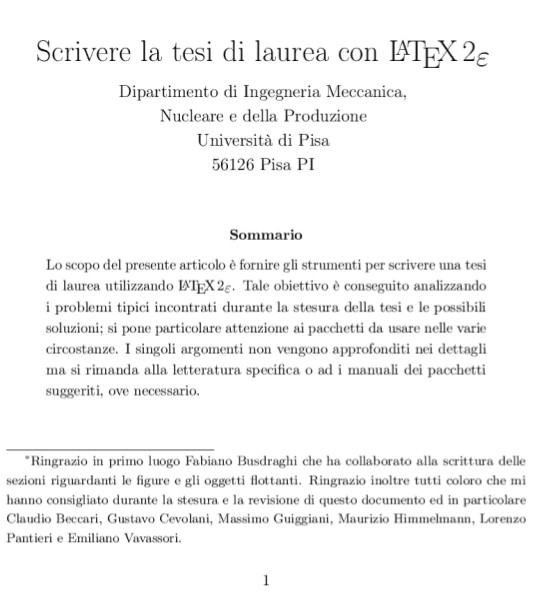
\includegraphics[width=.7\textwidth]{imgs/LatexDoc.jpg}
	\end{center}

\end{frame}

\begin{frame}
	\frametitle{I linguaggi di codifica}
	\framesubtitle{Linguaggi di marcatura dichiarativi}
	\addtocounter{nframe}{1}

	\begin{block}{Linguaggi dichiarativi}
		Orientati al testo, annotano la struttura, la funzione ed il significato degli elementi costitutivi
		del testo, tralasciandone l’aspetto.
		\begin{itemize}
			\item La posizione che il brano in questione occupa all’interno del documento (markup strutturale)
			\item Peculiarità del testo stesso (markup semantico)
			\item I fogli di stile definiscono la formattazione dell’output
			\item Molteplici usi del medesimo testo
		\end{itemize}
	\end{block}
    \textit{Esempio: famiglia SGML, XML}
	
\end{frame}

\begin{frame}
	\frametitle{I linguaggi di codifica}
	\framesubtitle{Linguaggi di marcatura dichiarativi}
	\addtocounter{nframe}{1}

	\begin{block}{Markup dichiarativi: contenuto e presentazione}
		La separazione tra contenuto e presentazione non solo è intenzionale, ma è la caratteristica principale di questi sistemi di marcatura: essa permette di concentrarsi sull'annotazione logica-semantica per funzioni di ricerca e di analisi, lasciando ad altro (ai fogli di stile) la resa grafica.
	\end{block}

	\begin{block}{Unico testo più usi}
		In questo modo si ha inoltre la possibilità di utilizzare uno stesso testo codificato con
		finalità o formattazioni differenti, a seconda delle varie esigenze.
	\end{block}

\end{frame}

\begin{frame}
	\frametitle{I linguaggi di codifica}
	\framesubtitle{Markup dichiarativi: esempio SGML}
	\addtocounter{nframe}{1}

	\begin{block}{Standard Generalized Markup Language}
		\begin{center}
			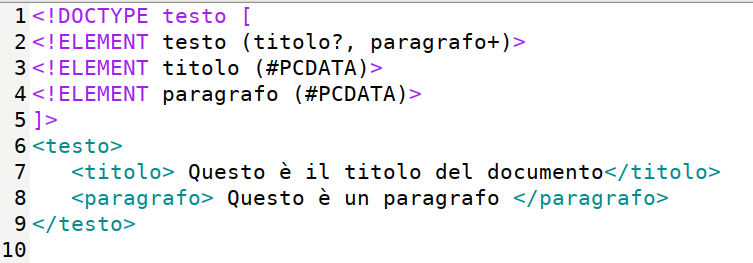
\includegraphics[width=.9\textwidth]{imgs/testo-sgml.png}
		\end{center}
	\end{block}

\end{frame}

\begin{frame}
	\frametitle{I linguaggi di codifica}
	\framesubtitle {Markup dichiarativi vs Markup procedurali}
	\addtocounter{nframe}{1}
	\begin{block}{resa a video della frase}
		Le \textit{Guidelines for Electronic Text Encoding and Interchange} sono \textit{molto} complete e descrivono uno standard di \textit{markup} del testo basato su XML.
	\end{block}

	\begin{center}
		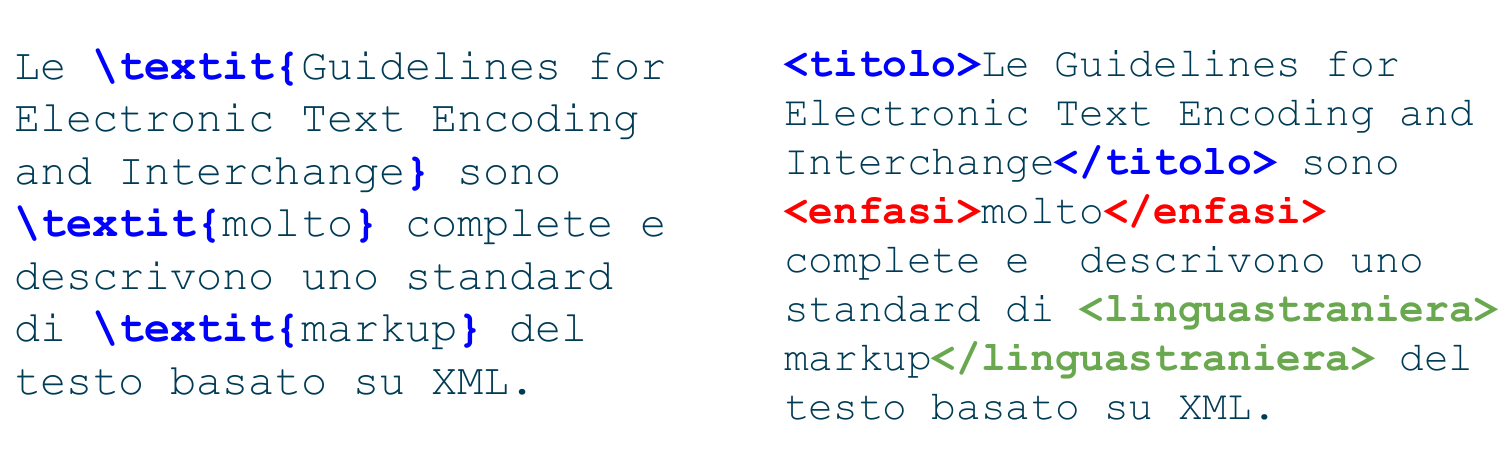
\includegraphics[width=.85\textwidth]{imgs/Procedurale-Dichiarativo.png}
	\end{center}
    \begin{center}
    \textbf{LaTex vs SGML}
    \end{center}

\end{frame}

\begin{frame}
	\frametitle{I linguaggi di codifica}
	\framesubtitle{Linguaggi di marcatura}
	\addtocounter{nframe}{1}

	\begin{block}{linguaggi semi-dichiarativi e/o semi-procedurali}
		Esistono anche linguaggi che possono essere definiti
		semi-procedurali, o semi-dichiarativi, che come si intuisce utilizzano le istruzioni sia
		per una codifica di tipo procedurale, sia per una codifica di tipo descrittivo o
		dichiarativo.
	\end{block}

	\begin{block}{HTML}
		HTML ha tra le sue etichette istruzioni di tipo procedurale per indicare come devono essere rese determinate
		porzioni di testo, e istruzioni di tipo dichiarativo che hanno una base semantica.
	\end{block}



\end{frame}


\section{Fondamenti del linguaggio XML}
%slide relative ad introdurre gli elementi di XML

% prendere da libro XML in amazon e XML visual quick view
% inserire qualche nota sul namespace anche preso dal libro xsd da pag 26 
% riprendere qualche slide dall slide Del Turco; e dalle slide Fiormonte-Ciotti-Silvi-XML-corso-2014.pdf
% http://filologiadigitale-verona.it/wp-content/uploads/2014/10/Fiormonte-Ciotti-Silvi-XML-corso-2014.pdf
% Slide Chiara di Pietro

% IDE/Editor comes with a nice XML/XSD editor. It has a number of features that makes schema writing lot easier. Intellisense, auto-completion, real-time syntax checks, etc., are a few of those features.

\begin{frame}
	\frametitle{Fondamenti XML}
	\framesubtitle{eXtensible Markup Language}
	\addtocounter{nframe}{1}

	\begin{block}{XML origini}
		XML affonda le proprie origini nel linguaggio Standard Generalized Markup Language (SGML).
		\\ SGML è stato introdotto negli anni ottanta con il fine di descrivere la struttura e il contenuto di qualsiasi informazione ``machine readable''.
	\end{block}

	\begin{block} {XML è una semplificazione di SGML}
		XML può essere pensato come una versione semplificata di SGML. Infatti, come SGML, XML è un meta-linguaggio, usato per create linguaggi di marcatura (detti vocabolari).
	\end{block}
\end{frame}

\begin{frame}
	\frametitle{Fondamenti XML}
	\framesubtitle{eXtensible Markup Language}
	\addtocounter{nframe}{1}

	\begin{block}{XML come meta-linguaggio}
		XML è un insieme di regole per definire linguaggi di marcatura personalizzati e personalizzabili (\textit{custom-built vocabolaries}).
	\end{block}

	\begin{block} {Applicazioni XML}
		Allo stesso modo di SGML, XML è nato per strutturare, conservare e trasportare informazioni.
		\\ I linguaggi di marcatura derivati da XML per strutturare e descrivere specifiche informazioni vengono chiamati \textit{XML applications} oltre a \textit{vocabolario XML}.
	\end{block}
\end{frame}

\begin{frame}
	\frametitle{Fondamenti XML}
	\framesubtitle{eXtensible Markup Language}
	\addtocounter{nframe}{1}

	\begin{block}{XML: eXtensible}
		XML è estensibile: è pensato per essere modificato ed esteso al fine di soddisfare le varie necessità di rappresentazione dell'informazione.
		\textbf{XML non contempla un vocabolario predefinito!}
	\end{block}

	\begin{block} {XML: standard W3C}
		XML è sviluppato e manutenuto dal W3C (World Wide Web Consortium), il quale sviluppa protocolli e standard riconosciuti dalla comunità scientifica e tecnica al fine di condividere informazioni sul Web..
	\end{block}
\end{frame}

\begin{frame}
	\frametitle{Fondamenti XML}
	\framesubtitle{eXtensible Markup Language}
	\addtocounter{nframe}{1}

	\begin{block}{XML: riassumendo}
		XML, eXtensible Markup Language, derivato dal SGML, , 
		è una specificazione, un formalismo, per conservare e scambiare informazioni in formato machine redable (digitale).
	\end{block}

	\begin{block}{XML: riassumendo}
		XML è anche una specificazione per descrivere la struttura dell'informazione seguendo un modello dei dati gerarchico.
		\\ XML è simile ad HTML, ma a differenza di questo non ha etichette predefinite.
	\end{block}

\end{frame}


\begin{frame}
	\frametitle{Fondamenti XML}
	\framesubtitle{eXtensible Markup Language}
	\addtocounter{nframe}{1}

	\begin{center}
		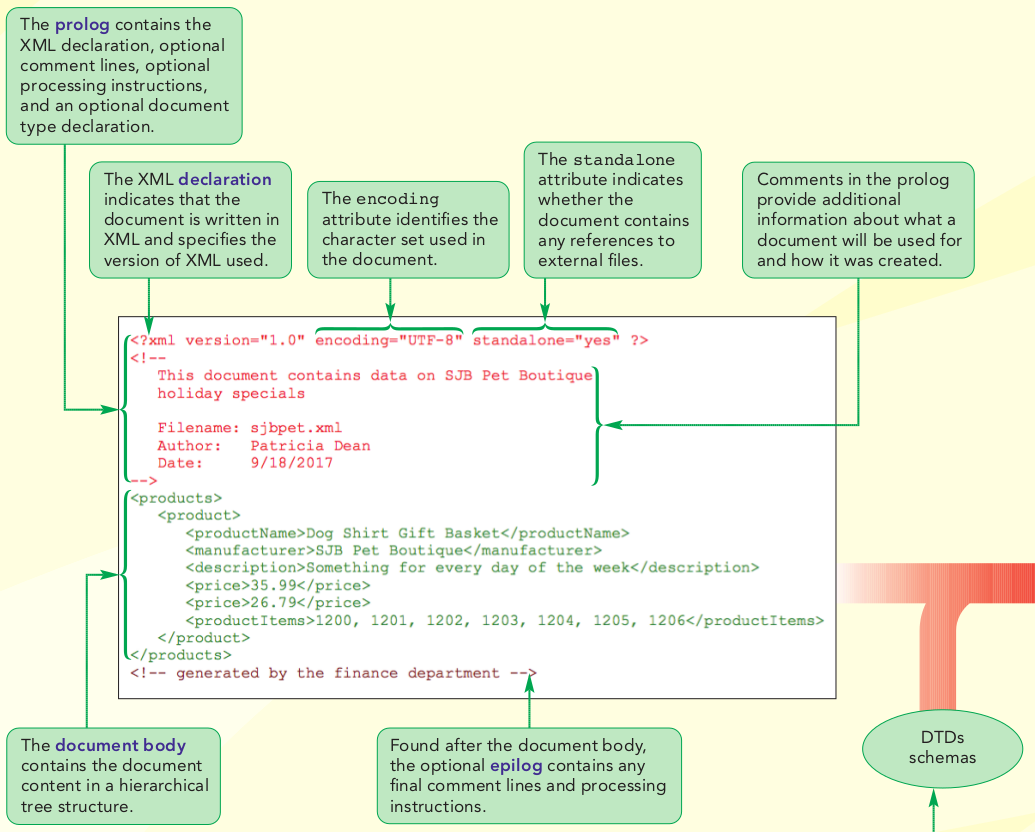
\includegraphics[width=.8\textwidth]{imgs/xml-intro-doc-xml.png}
	\end{center}

	\begin{tiny}\textit{immagine dal libro New Perspectives on XML, 3rd Edition}\end{tiny}

\end{frame}


%The syntax rules of XML are easy to learn and easy to use
\begin{frame}
	\frametitle{Fondamenti XML}
	\framesubtitle{eXtensible Markup Language: regole sintattiche}
	\addtocounter{nframe}{1}

	\begin{itemize}

		\item Ciascun elemento XML deve avere un tag di chiusura.
			%Every XML element must have a closing tag.
		      %Every element must have a closing tag. A self-closing tag is permitted.

		\item I tag XML sono \textit{case sensitive}.
			%XML tags are case sensitive.
		      % Opening and closing tags (or start and end tags) must be ­written with the same case.

		\item Gli elementi XML devono essere annidati in modo rigoroso.
			%XML elements must be ­properly nested.
		      %All elements can have child (sub) elements. Child elements must be in pairs and be correctly nested within their respective parent element.

		\item Tutti i documenti XML deveno avere un elemento radice (root) che contiene tutti gli altri elementi opportunamente annidati.
			%Every XML document must have a root element.
		      %Every XML document must contain a single tag pair that defines the root element. All other elements must be nested within the root element.

		\item Gli elementi XML possono avere attributi con stile nome-valore.
		
	\end{itemize}

\end{frame}


%The syntax rules of XML are easy to learn and easy to use 2
\begin{frame}
	\frametitle{Fondamenti XML}
	\framesubtitle{eXtensible Markup Language: regole sintattiche cont.}
	\addtocounter{nframe}{1}

	\begin{itemize}
		\item Un attributo all'interno dell'elemento può apparire una sola volta
		
		\item Il valore degli attributi è una stringa e deve essere inserita tra apici
			%XML elements can have attributes in name-value pairs.
		      %Each attribute name within the same element can occur only once.% Each attribute value must be quoted.

		\item Esistono alcuni caratteri spciali che non possono essere usati. 
			%Some characters have a ­special meaning in XML.
		      %The use of certain characters is restricted. If these characters are needed, entity references or character references may be used. References always begin with the character “&” (which is ­specially reserved) and end with the character “;”.

		      %XML allows for comments. 
		\item I commenti non possono essere inseriti prima della dichiarazione XML e non possono essere annidati.
			%Comments cannot occur prior to the XML Declaration. Comments cannot be nested.

	\end{itemize}

\end{frame}

\begin{frame}
	\frametitle{Fondamenti XML}
	\framesubtitle{eXtensible Markup Language}
	\addtocounter{nframe}{1}

	\begin{block}{Manutenibilità}
		Data la semplicità delle regole e della sintassi XML incentrata sulla memorizzazione e scambio dei dati, la struttura generale di un documento XML è semplice sia dal punto di vista della progettazione sia dal punto di vista della manutenibilità.
	\end{block}

\end{frame}

\begin{frame}
	\frametitle{Fondamenti XML}
	\framesubtitle{eXtensible Markup Language}
	\addtocounter{nframe}{1}

	\begin{block}{XML vista ad albero}
		XML ha un modello dei dati gerarchico e può quindi essere visto come un albero ordinato.
		\\Per questo motivo le informazioni sono rappresentate in modo ottimale se sono gerarchiche e sequenziali.
	\end{block}

\end{frame}


\begin{frame}
	\frametitle{Fondamenti XML}
	\framesubtitle{eXtensible Markup Language: vista ad albero}
	\addtocounter{nframe}{1}

	\begin{center}
		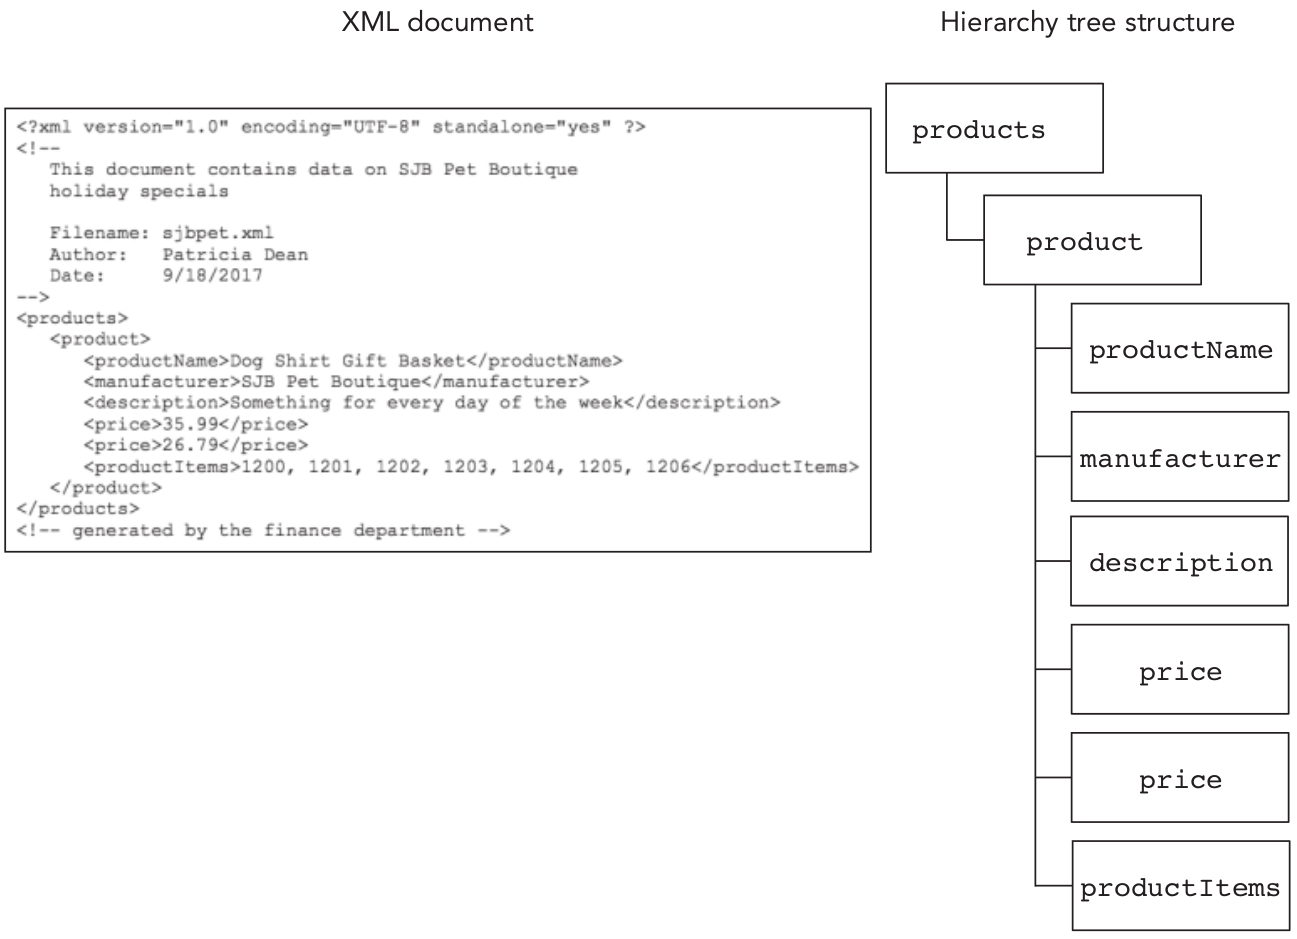
\includegraphics[width=.9\textwidth]{imgs/XML-TreeStructure.png}
	\end{center}

\begin{tiny}\textit{immagine dal libro New Perspectives on XML, 3rd Edition}\end{tiny}

\end{frame}

\begin{frame}
	\frametitle{Fondamenti XML}
	\framesubtitle{eXtensible Markup Language}
	\addtocounter{nframe}{1}

	\begin{block}{TEI-XML vocabulary}
		Al fine di soddisfare i requisiti degli studiosi del testo il vocabolario TEI-XML è stato sviluppato nel corso degli ultimi decenni con lo scopo e l'obiettivo di permettere la codifica di qualsiasi informazione testuale.
	\end{block}
	
	\textit{Un vocabolario XML è un insieme di tag XML sviluppato per una particolare esigenza di codifica}

\end{frame}


\begin{frame}
	\frametitle{Fondamenti XML}
	\framesubtitle{eXtensible Markup Language: Esempio TEI}
	\addtocounter{nframe}{1}

	\begin{center}
		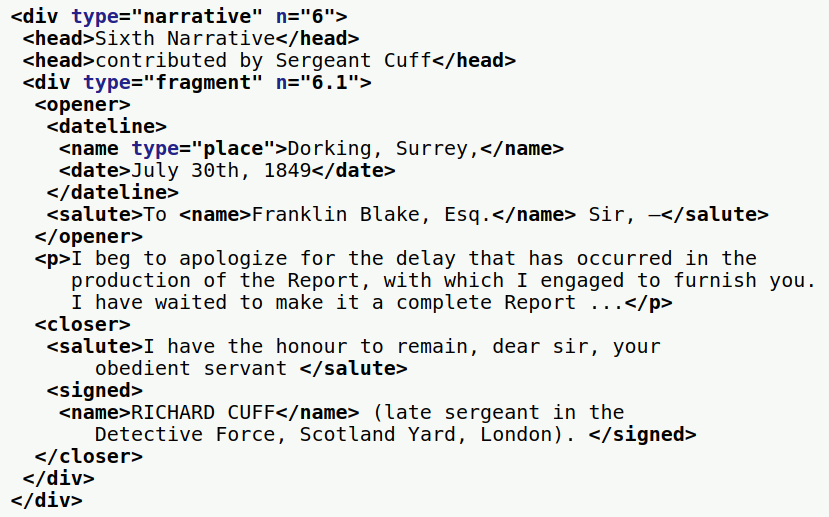
\includegraphics[width=.9\textwidth]{imgs/xml-TEI-Example.png}
	\end{center}

	\begin{tiny}
        \textit{immagine dal sito TEI Guide Lines}
    \end{tiny}

\end{frame}


\begin{frame}
	\frametitle{Fondamenti XML}
	\framesubtitle{eXtensible Markup Language}
	\addtocounter{nframe}{1}

	\begin{block}{Documento ben formato (well-formed)}
		Un documento XML deve essere ben formato (well-formed), cioè non deve contenere errori sintattiti e soddisfare le regole generali della specifica.
	\end{block}
	\textit{Un documento non ben formato non può essere letto dalle applicazioni che elaborano codice XML}.

\end{frame}


\begin{frame}
	\frametitle{Fondamenti XML}
	\framesubtitle{eXtensible Markup Language}
	\addtocounter{nframe}{1}

	\begin{block}{Parti principali di un documento XML}
		Un documento XML consiste di tre parti:
		\begin{itemize}
			\item il prologo
			\item il corpo (body)
			\item l'epilogo
		\end{itemize}
	\end{block}

\end{frame}


\begin{frame}
	\frametitle{Fondamenti XML}
	\framesubtitle{eXtensible Markup Language: Esempio TEI}
	\addtocounter{nframe}{1}

	\begin{center}
		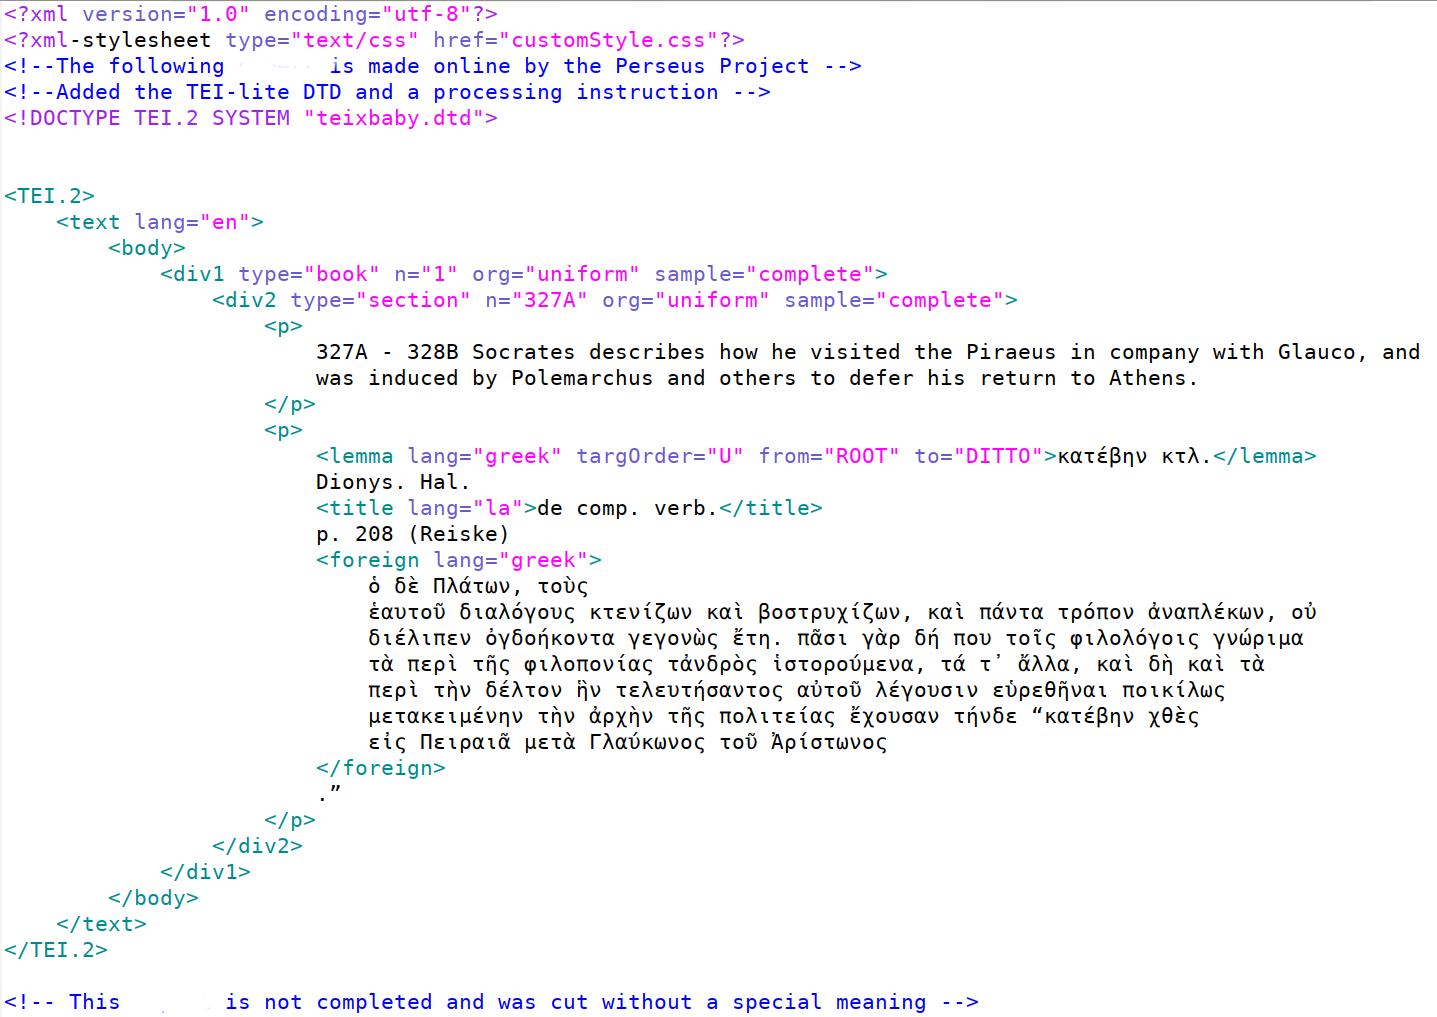
\includegraphics[width=0.95\textwidth]{imgs/xml-TEI-PerseusExample.png}
	\end{center}

\end{frame}


\begin{frame}
	\frametitle{Fondamenti XML}
	\framesubtitle{eXtensible Markup Language}
	\addtocounter{nframe}{1}

	\begin{block}{Documento XML: prologo}
		\begin{itemize}
			\item XML declaration (obbligatorio)
			\item Processing instructions (opzionale)
			\item Commenti (opzionale)
			\item Document type declaration (opzionale)
		\end{itemize}
        
        % XML declaration: indicates that the document is written in the XML language
        % Processing instructions (optional): provide additional instructions to be run by programs that read the XML document
        % Comment lines (optional): provide additional information about the document contents
        % Document type declaration (DTD) (optional): provides information about the rules used in the XML document’s vocabulary
	\end{block}

\end{frame}

\begin{frame}
	\frametitle{Fondamenti XML}
	\framesubtitle{eXtensible Markup Language}
	\addtocounter{nframe}{1}

	\begin{block}{Documento XML: corpo}
		Il corpo del documento XML segue immediatamente il prologo. Questa parte del documento contiene il contenuto vero e proprio in una struttura ad albero ordinata.
	\end{block}

	\begin{block}{Documento XML: epilogo}
		Opzionalmente, al corpo del documento XML segue un epilogo il quale può contenere commenti finale e processing instructions.
	\end{block}
	

\end{frame}

\begin{frame}
	\frametitle{Fondamenti XML}
	\framesubtitle{eXtensible Markup Language: Prologo}
	\addtocounter{nframe}{1}

	\begin{block}{XML declaration}
    \begin{center}\texttt{<?xml version=”version number” encoding=”encoding type” standalone=”yes|no” ?>}\end{center}
	\end{block}

\end{frame}

% Creating an XML Declaration
% • To create an XML declaration, enter the code
% <?xml ?>
% in the first line of an XML document.
% • To specify a version of XML to use, enter the code
% version=”version number”
% after the opening <?xml tag, where version number is either 1.0 or 1.1.
% • To specify a character encoding, enter the code
% encoding=”encoding type”
% after the version attribute-value pair, where encoding type identifies the ­character
% set used in the document.
% • To indicate whether the document is a standalone document, enter the code
% standalone=”yes|no”
% after the encoding attribute-value pair, where the value yes or no ­indicates whether
% access to external files will be needed when processing the document.

\begin{frame}
	\frametitle{Fondamenti XML}
	\framesubtitle{eXtensible Markup Language: Prologo}
	\addtocounter{nframe}{1}

	\begin{block}{XML declaration: ERRORI}
	\begin{center}\texttt{<?XML VERSION=”1.0” ENCODING=”ISO-8859-1” STANDALONE=”YES” ?>}\end{center}
	\begin{center}\texttt{<?xml version=1.0 encoding=ISO-8859-1 standalone=yes ?>}\end{center}
	\begin{center}\texttt{<?xml version=”1.0” standalone=”yes” encoding=”ISO-8859-1” ?>}\end{center}
	\end{block}

\end{frame}

\begin{frame}
	\frametitle{Fondamenti XML}
	\framesubtitle{eXtensible Markup Language: Prologo}
	\addtocounter{nframe}{1}

	\begin{block}{XML comments}
		I commenti XML vengono ignorati dai programmi che elaborano il documento.
		\\I commenti quindi non influenzano i contenuti e la sruttura del documento.
	\end{block}

	\begin{block}{XML comments: sintassi}
	\begin{center}\texttt{
		<!-- il parser XML qui non entra -->
	}\end{center}
	\end{block}

	\textit{Un commento può occupare anche più righe}
	
\end{frame}

\begin{frame}
	\frametitle{Fondamenti XML}
	\framesubtitle{eXtensible Markup Language}
	\addtocounter{nframe}{1}

	\begin{center}
		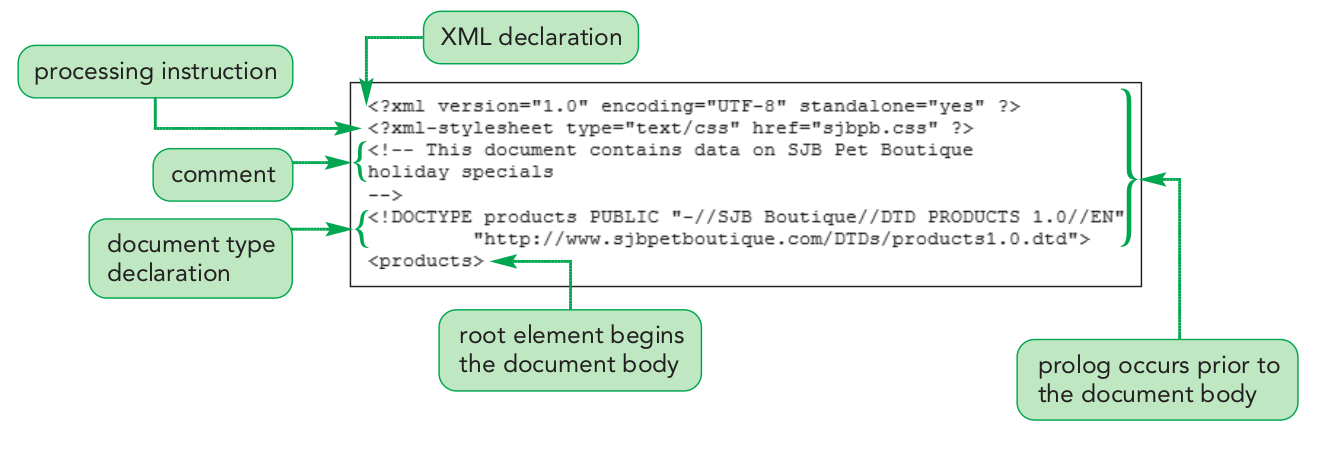
\includegraphics[width=0.95\textwidth]{imgs/XML-Prologo.png}
    \end{center}
\begin{tiny}\textit{immagine dal libro New Perspectives on XML, 3rd Edition}\end{tiny}

\end{frame}

\begin{frame}
	\frametitle{Fondamenti XML}
	\framesubtitle{eXtensible Markup Language}
	\addtocounter{nframe}{1}

	\begin{block}{Esercizio prologo}
		Creare un file \textit{.xml} ed inserire un prologo con la dichiarazione XML e un commento con le vostre informazioni.
	\end{block}

	\begin{block}{Esercizio prologo}
		\texttt{
		 <!--
		 	This document contains data on Codifica di Testi.
		 	\\Filename: project.xml
		 	\\Author: your name
		 	\\Date: today's date
		-->
		}
	\end{block}

	\begin{tiny}
		\textit{Salvare il file su github nel repository del progetto}
	\end{tiny}

\end{frame}

\begin{frame}
	\frametitle{Fondamenti XML}
	\framesubtitle{eXtensible Markup Language}
	\addtocounter{nframe}{1}

	\begin{block}{XML parser}
		Un programma che legge ed interpreta un documento XML è chiamato XML parser ( o processor).
	\end{block}
	\begin{block}{Cosa fa un XML parser}
		\begin{itemize}
			\item Verifica che il documento rispetti la  XML
			\item Interpreta i dati con tipo PCDATA 
			\item Risolve character or entity references
			\item Gestisce le processing instructions per interpretare i dati
		\end{itemize}
	\end{block}

\end{frame}

\begin{frame}
	\frametitle{Fondamenti XML}
	\framesubtitle{eXtensible Markup Language}
	\addtocounter{nframe}{1}

	\begin{block}{XMLlint}
		\begin{center}
			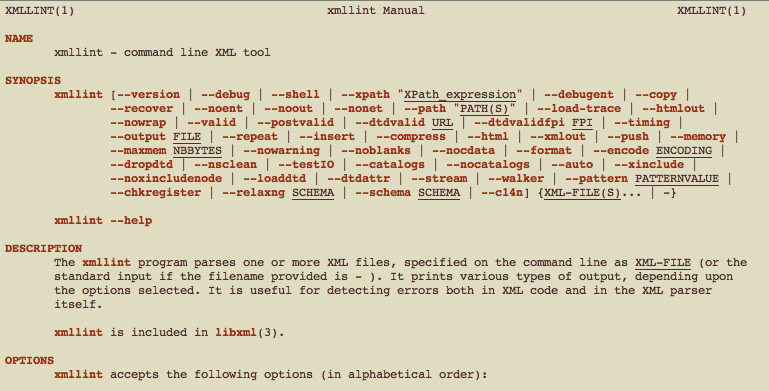
\includegraphics[width=0.95\textwidth]{imgs/xml-XMLlint-man.png}
		\end{center}
	\end{block}

\end{frame}


\begin{frame}
    \frametitle{Fondamenti XML}
    \framesubtitle{eXtensible Markup Language}
    \addtocounter{nframe}{1}

	\begin{block}{XML body}
		Un documento XML è composto da elementi e attributi. 
	   \\ Gli elementi sono la base, le unità fondamentali di qualsiasi documento XML.
    \end{block}

    \begin{block}{Elementi: Sintassi}
    \begin{center}\texttt{<element>content</element>}\end{center}
    \begin{center}\texttt{opening tag: <element>;\\ closing tag: </element>}\end{center}
	\end{block}
	\begin{tiny}
		\textit{Un elemento può contenere testo e/o ulteriori elementi}
	\end{tiny}
	
\end{frame}

\begin{frame}
    \frametitle{Fondamenti XML}
    \framesubtitle{eXtensible Markup Language}
    \addtocounter{nframe}{1}

	\begin{block}{XML Element}
		\textit{Gli elementi XML possono avere diversi tipi di contenuto}:
		\begin{itemize}
			\item contenuto strutturale: solo altri elementi, non testo
			\item contenuto misto: testo e anche altri elementi
			\item contenuto testuale: solo testo, non altri elementi
		\end{itemize}
	\end{block}
	
\end{frame}

\begin{frame}
    \frametitle{Fondamenti XML}
    \framesubtitle{eXtensible Markup Language}
    \addtocounter{nframe}{1}

	\begin{block}{XML Element: note importanti sul nome}
		\begin{itemize}
			\item Gli elementi sono case sensitive.
			\item Gli elementi possono iniziare con una lettera o con un ``\_''.
			\item Un elemento non può iniziare con la stringa \textit{xml}. 
			\item Il tag di apertura e di chiusura devono avere lo stesso nome.
			\item Un tag può essere usato più di una volta.
			\item Un insieme di elementi costituiscono un vocabolario
		\end{itemize}
	\end{block}
\end{frame}




% There are a few important points to remember about XML elements:
% • Element names are case sensitive, which means that, for example, itemnumber,
% itemNumber, and ItemNumber are unique elements.
% • Element names must begin with a letter or the underscore character ( \_ ) and may not
% contain blank spaces. Thus, you cannot name an element Item Number , but you can
% name it Item\_Number .
% • Element names cannot begin with the string xml because that group of ­characters is
% reserved for special XML commands.
% • The name in an element’s closing tag must exactly match the name in the ­opening tag.
% • Element names can be used more than once, so the element names can mean
% different things at different points in the hierarchy of an XML document.

% Element names might be established already if an author is using a particular XML
% vocabulary, such as TEI-XML

% Creating XML Elements
% XML 24
% • To create an XML element, use the syntax
% <element>content</element>
% where element is the name given to the element, content represents the text
% content of the element, <element> is the opening tag, and <
% ­ /element> is the
% closing tag.
% • To create an empty XML element with a single tag, use the following syntax:
% <element />
% • To create an empty XML element with a pair of tags, use the syntax
% <element></element>

\begin{frame}
    \frametitle{Fondamenti XML}
    \framesubtitle{eXtensible Markup Language}
    \addtocounter{nframe}{1}

	\begin{block}{XML Element: empty e nested}
		\begin{itemize}
			\item Un elemento vuoto (\textit{empty}) è un elemento senza contenuto.
			\item Un elemento può contenere altri elementi opportunamente annidati (\textit{nested element}).
		\end{itemize}
	\end{block}

	\begin{block}{XML esempi: empty e nested element}
		\begin{itemize}
			\item \texttt{<element />} \texttt{<element></element>}
			\item \texttt{<choice><sic>testo con errore</sic><cor> testo corretto</cor></choice>}
		\end{itemize}
		
	\end{block}
	
\end{frame}


% ESEMPIO
% <product>
% <productName>Dog Shirt Gift Basket</productName>
% <manufacturer>SJB Pet Boutique</manufacturer>
% <description>Something for every day of the week</description>
% <price>35.99</price>
% <price>26.79</price>
% <productItems>1200, 1201, 1202, 1203, 1204, 1205, 1206
% </productItems>
% </product>

\begin{frame}
    \frametitle{Fondamenti XML}
    \framesubtitle{eXtensible Markup Language}
    \addtocounter{nframe}{1}

	\begin{block}{XML Element: hierarchical relationship}
		\begin{itemize}
			\item Un elemento annidato (\textit{nested}) è un elemento \textit{figlio}, cioè contenuto (annidato) in un ulteriore elemento detto padre/genitore (\textit{parent}).
			\item Gli elementi che sono presenti su uno stesso livello gerarchiso (\textit{side by side}) sono detti \textit{sibling element}.
		\end{itemize}
	\end{block}

\end{frame}

\begin{frame}
	\frametitle{Fondamenti XML}
	\framesubtitle{eXtensible Markup Language}
	\addtocounter{nframe}{1}

	\begin{center}
		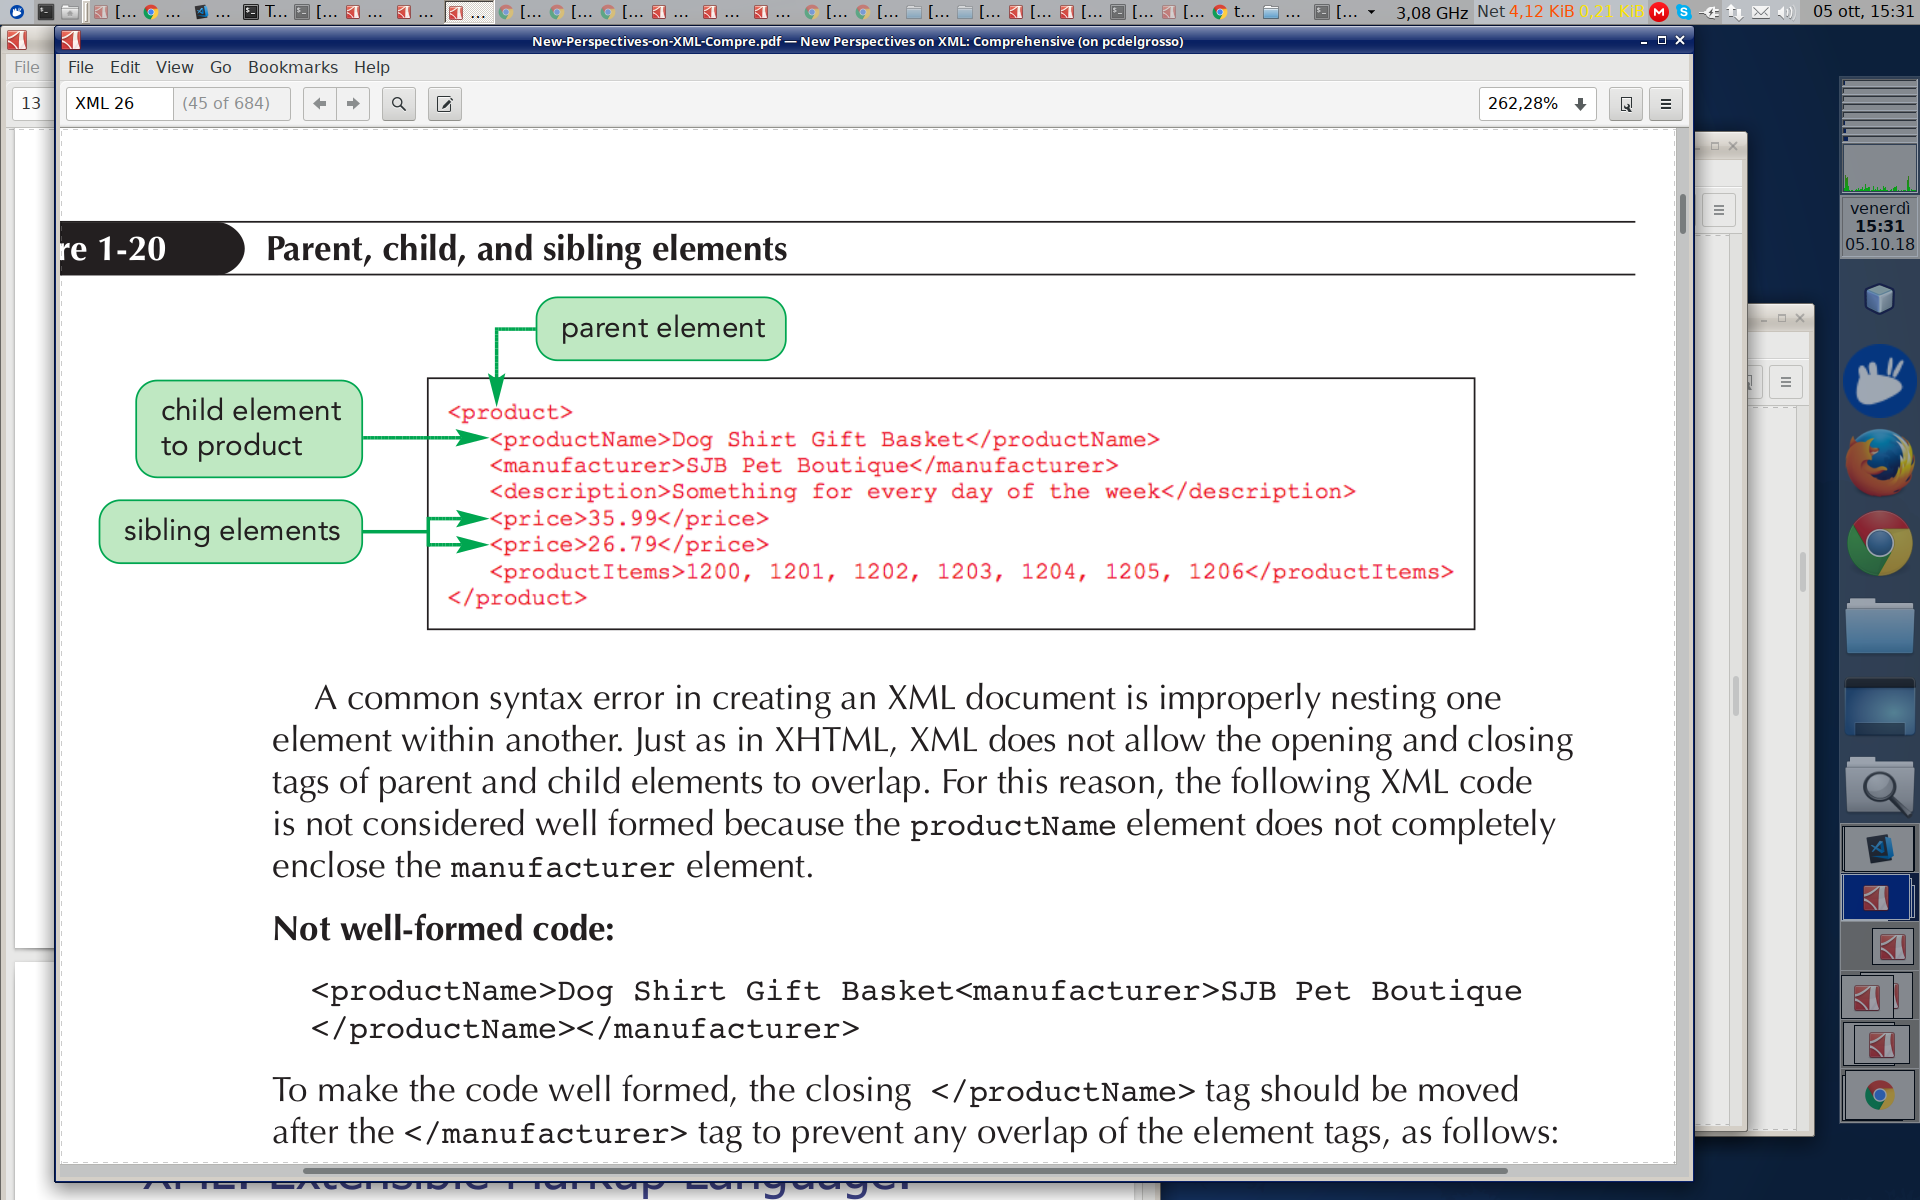
\includegraphics[width=0.95\textwidth]{imgs/XML-Parent-Child-Sibling.png}
    \end{center}
\begin{tiny}\textit{immagine dal libro New Perspectives on XML, 3rd Edition}\end{tiny}

\end{frame}

\begin{frame}
    \frametitle{Fondamenti XML}
    \framesubtitle{eXtensible Markup Language}
    \addtocounter{nframe}{1}

	\begin{block}{XML Element: hierarchical relationship}
		\begin{itemize}
			\item Tutti gli elementi nel body del documento sono figli di uno stesso elemento, chiamato radice (\textit{root}).
			\item Un documento XML deve contenere un elemento root per essere considerato ben formato.
			\item Una gerarchia XML può essere rappresentata tramite un diagramma ad albero.
		\end{itemize}
	\end{block}

\end{frame}

\begin{frame}
    \frametitle{Fondamenti XML}
    \framesubtitle{eXtensible Markup Language}
    \addtocounter{nframe}{1}

	\begin{block}{XML Element: hierarchical relationship cont.}
		\begin{itemize}
			\item Il prologo e i commenti non fanno parte dell'albero del body.
			\item Elementi non annidati correttamente implicano un errore di sintassi nei parser.
			\item Le specifiche XML non consentono di sovrapporre i tag di apertura e di chiusura degli elementi annidati (\textit{no overlap}).
		\end{itemize}
	\end{block}

\end{frame}


\begin{frame}
    \frametitle{Fondamenti XML}
    \framesubtitle{eXtensible Markup Language}
    \addtocounter{nframe}{1}

	\begin{block}{XML Element: hierarchical relationship - Esercizio}
		\begin{center}
			Scrivere e fare il check di un xml non opportunamente annidato
		\end{center}
	\end{block}

\end{frame}

% However, by indenting the code and placing siblings on their own lines, you can visually
% reveal the hierarchy relationships and add a dimension of visual communication to your
% code.

\begin{frame}
    \frametitle{Fondamenti XML}
    \framesubtitle{eXtensible Markup Language}
    \addtocounter{nframe}{1}

	\begin{block}{XML Element: hierarchical relationship as tree structure}
		Un modo rapido e comodo per visualizzare la struttura completa di un documento XML è quello di disegnare attraverso un diagramma ad albero ordinato gli elementi del documento XML.
	\end{block}

\end{frame}

% It would be useful to have a general tree diagram that indicates whether a particular
% child element can occur zero times, once, or several times within a parent

% The symbols ?, *, and + are part of the code used in creating DTDs to validate XML
% documents.

\begin{frame}
	\frametitle{Fondamenti XML}
	\framesubtitle{eXtensible Markup Language}
	\addtocounter{nframe}{1}

	\begin{center}
		%aggiornare immagine

		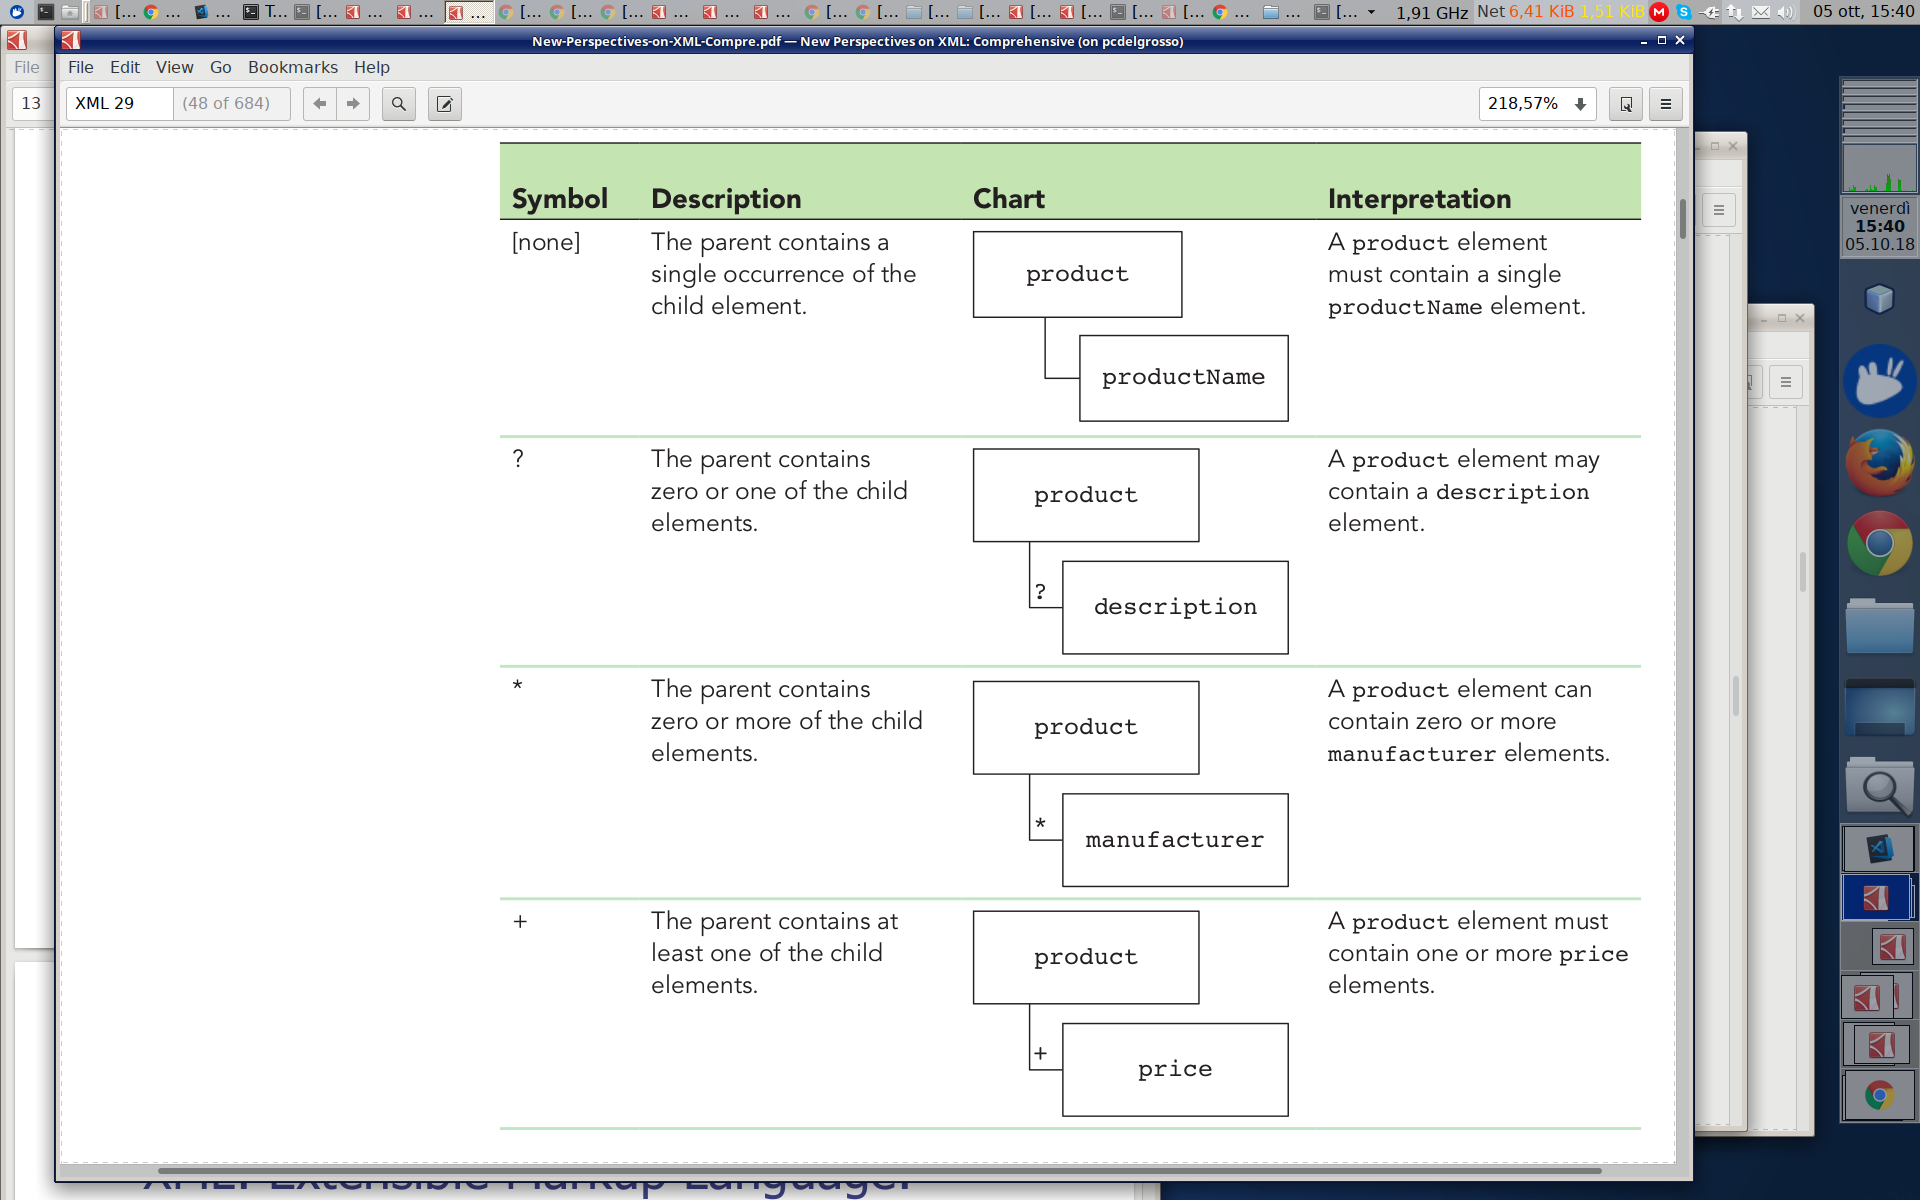
\includegraphics[width=0.8\textwidth]{imgs/xml-parent-child-quantifier.png}
    \end{center}
    
\begin{tiny}\textit{immagine dal libro New Perspectives on XML, 3rd Edition}\end{tiny}

\end{frame}

\begin{frame}
	\frametitle{Fondamenti XML}
	\framesubtitle{eXtensible Markup Language}
	\addtocounter{nframe}{1}

	\begin{center}
		
		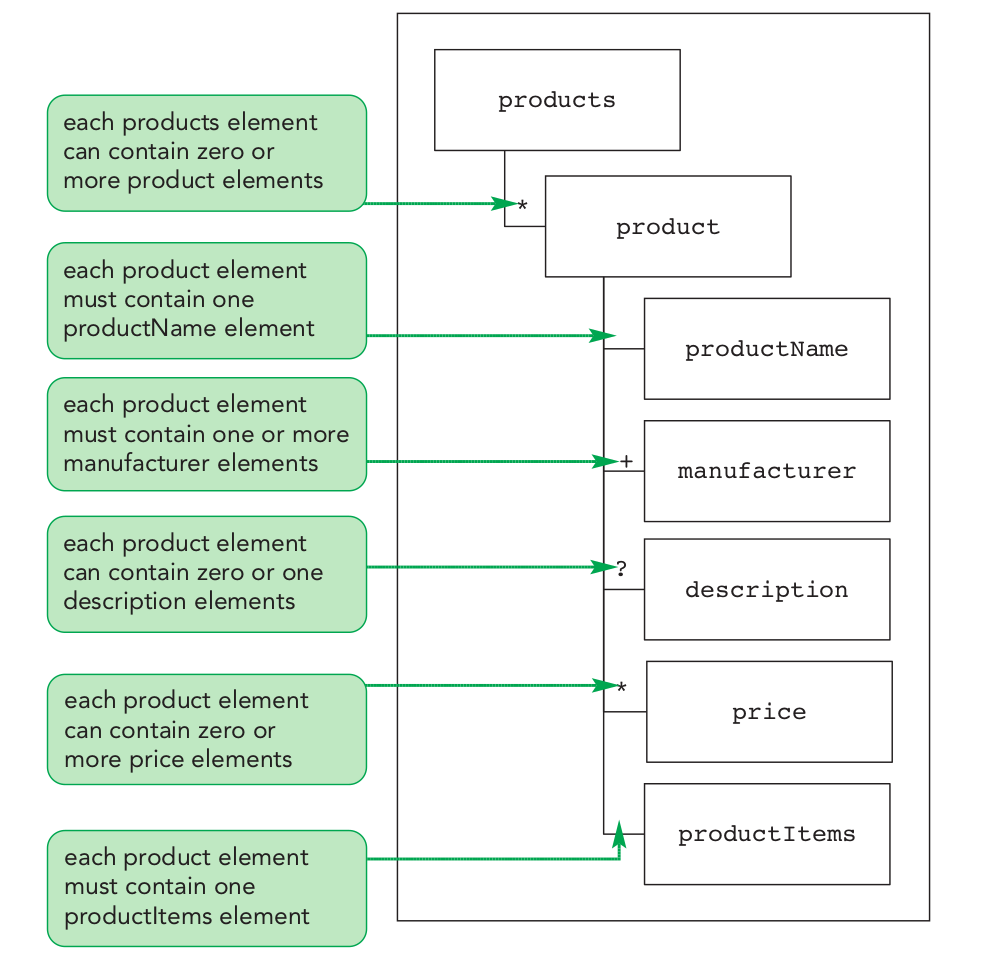
\includegraphics[width=0.8\textwidth]{imgs/xml-parent-child-quantifier2.png}
	\end{center}
\begin{tiny}\textit{immagine dal libro New Perspectives on XML, 3rd Edition}\end{tiny}
\end{frame}


\begin{frame}
    \frametitle{Fondamenti XML}
    \framesubtitle{eXtensible Markup Language}
    \addtocounter{nframe}{1}

	\begin{block}{XML Element: Mixed Content}
		Un elemento può contenere contemporaneamente sia testo sia altri elementi. 
		\\Questo modello di contenuto si chiama Mixed Content ed è ideale per descrivere informazioni text-based (\textbf{dati semi-strutturati)}.
	\end{block}

	\begin{block}{XML Element: Mixed Content}
		\texttt{
			<p><salutation>Salve</salutation> il mio nome è <persName>Angelo</persName></p>
			} 
	\end{block}


\end{frame}

\begin{frame}
    \frametitle{Fondamenti XML}
    \framesubtitle{eXtensible Markup Language}
    \addtocounter{nframe}{1}

	\begin{block}{XML Element: Esercizio}
		Aprire il file XML non ben formato presente nel repository github:
		\begin{itemize}
			\item validarlo con XMLlint
			\item correggerlo (commentando gli errori e le modifiche)
			\item aggiungere un figlio (child) ad un elemento
			\item aggiungere un fratello (sibling) ad un elemento
		\end{itemize}
	\end{block}

\end{frame}


\begin{frame}
    \frametitle{Fondamenti XML}
    \framesubtitle{eXtensible Markup Language}
    \addtocounter{nframe}{1}

	\begin{block}{XML Attributi}
		Gli elementi in un documento XML puossono avere uno o più attributi.
		\\ Un attributo descrive una caratteristica dell'elemento in cui appare.
	\end{block}

	\begin{block}{XML Attributi}
		Un attributo ha senso solo all'interno del proprio elemento e non è possibile separarlo da esso in alcun modo.
	\end{block}

\end{frame}


\begin{frame}
    \frametitle{Fondamenti XML}
    \framesubtitle{eXtensible Markup Language}
    \addtocounter{nframe}{1}

	\begin{block}{XML Attributi: valore}
		Un attributo ha due componenti: nome - valore.
		Il valore di un attributo è una stringa e deve essere sempre racchiusa tra apici (singoli o doppi).
	\end{block}

	\begin{block}{XML Attributi: valore}
		\begin{center}
			\texttt{<element attribute=``value''> ... </element>}
			\\\texttt{<element attribute=``value'' />}
			\\\texttt{<element attribute=``value'', attribute2=``value2'' />}
		\end{center}
	\end{block}

\end{frame}

\begin{frame}
    \frametitle{Fondamenti XML}
    \framesubtitle{eXtensible Markup Language}
    \addtocounter{nframe}{1}

	\begin{block}{XML Attributi: restrizioni ai nomi}
		\begin{itemize}
			\item Il nome di un attributo può iniziare con una lettera oppure underscore.
			\item Gli spazi non sono consentiti in un nome di un attibuto.
			\item Il nome di un attributo non pò iniziare con la stringa \textit{xml}.
		\end{itemize}
	\end{block}

	\begin{block}{XML Attributi}
		\begin{itemize}
			\item Il nome degli attributi è \textit{case sensitive}.
			\item L'ordine degli attributi non è significativo.
		\end{itemize}
	\end{block}

\end{frame}


% Esercizio con gli attributi:
% (preso dalla TEI)


% Adding an Attribute to an Element
% • To add an attribute to an element, use the syntax
% <element attribute=”value”> ... </element>
% where element is the name given to the element, attribute is the ­attribute’s
% name, and value is the attribute’s value.
% • To add an attribute to a single-sided tag, use the syntax
% <element attribute=”value” />
% • To specify multiple attributes for a single element, use the syntax
% <element attribute1=”value1” attribute2=”value2” ...> ... </element>
% where attribute1 is the first attribute’s name, value1 is the first attribute’s value,
% attribute2 is the second attribute’s name, value2 is the second ­attribute’s
% value, and so on. Each attribute is separated by a space.



% It’s not always clear when to use an attribute value rather than inserting a new element.
% A general rule of thumb is that if all of the XML tags and their attributes were
% removed from a document, the remaining text should comprise the document’s content
% or information.
% Another rule of thumb is that attributes should be used to describe data, but should
% not contain data themselves.
% Different developers have different preferences, and
% there’s no right answer.

\begin{frame}
    \frametitle{Fondamenti XML}
    \framesubtitle{eXtensible Markup Language}
    \addtocounter{nframe}{1}

	\begin{block}{XML Character and Entity References}
		\begin{itemize}
			\item numeric character reference: \&\#nnn;
			\item character entity reference: \&entity;
		\end{itemize}
	\end{block}

	\begin{block}{XML References}
		\begin{itemize}
			\item \texttt{\&\#65;} (\textit{carattere A})
			\item \texttt{\&amp;} (\textit{carattere \&})
		\end{itemize}
	\end{block}

\end{frame}

% Inserting Character and Entity References
% • To insert a character reference into an XML document, use
% \&\#nnn;
% where nnn is a character reference number from the ISO/IEC character set.
% • To insert an entity reference, use
% \&entity;
% where entity is a recognized entity name.

% Immagine
\begin{frame}
	\frametitle{Fondamenti XML}
	\framesubtitle{eXtensible Markup Language}
	\addtocounter{nframe}{1}

	\begin{center}
			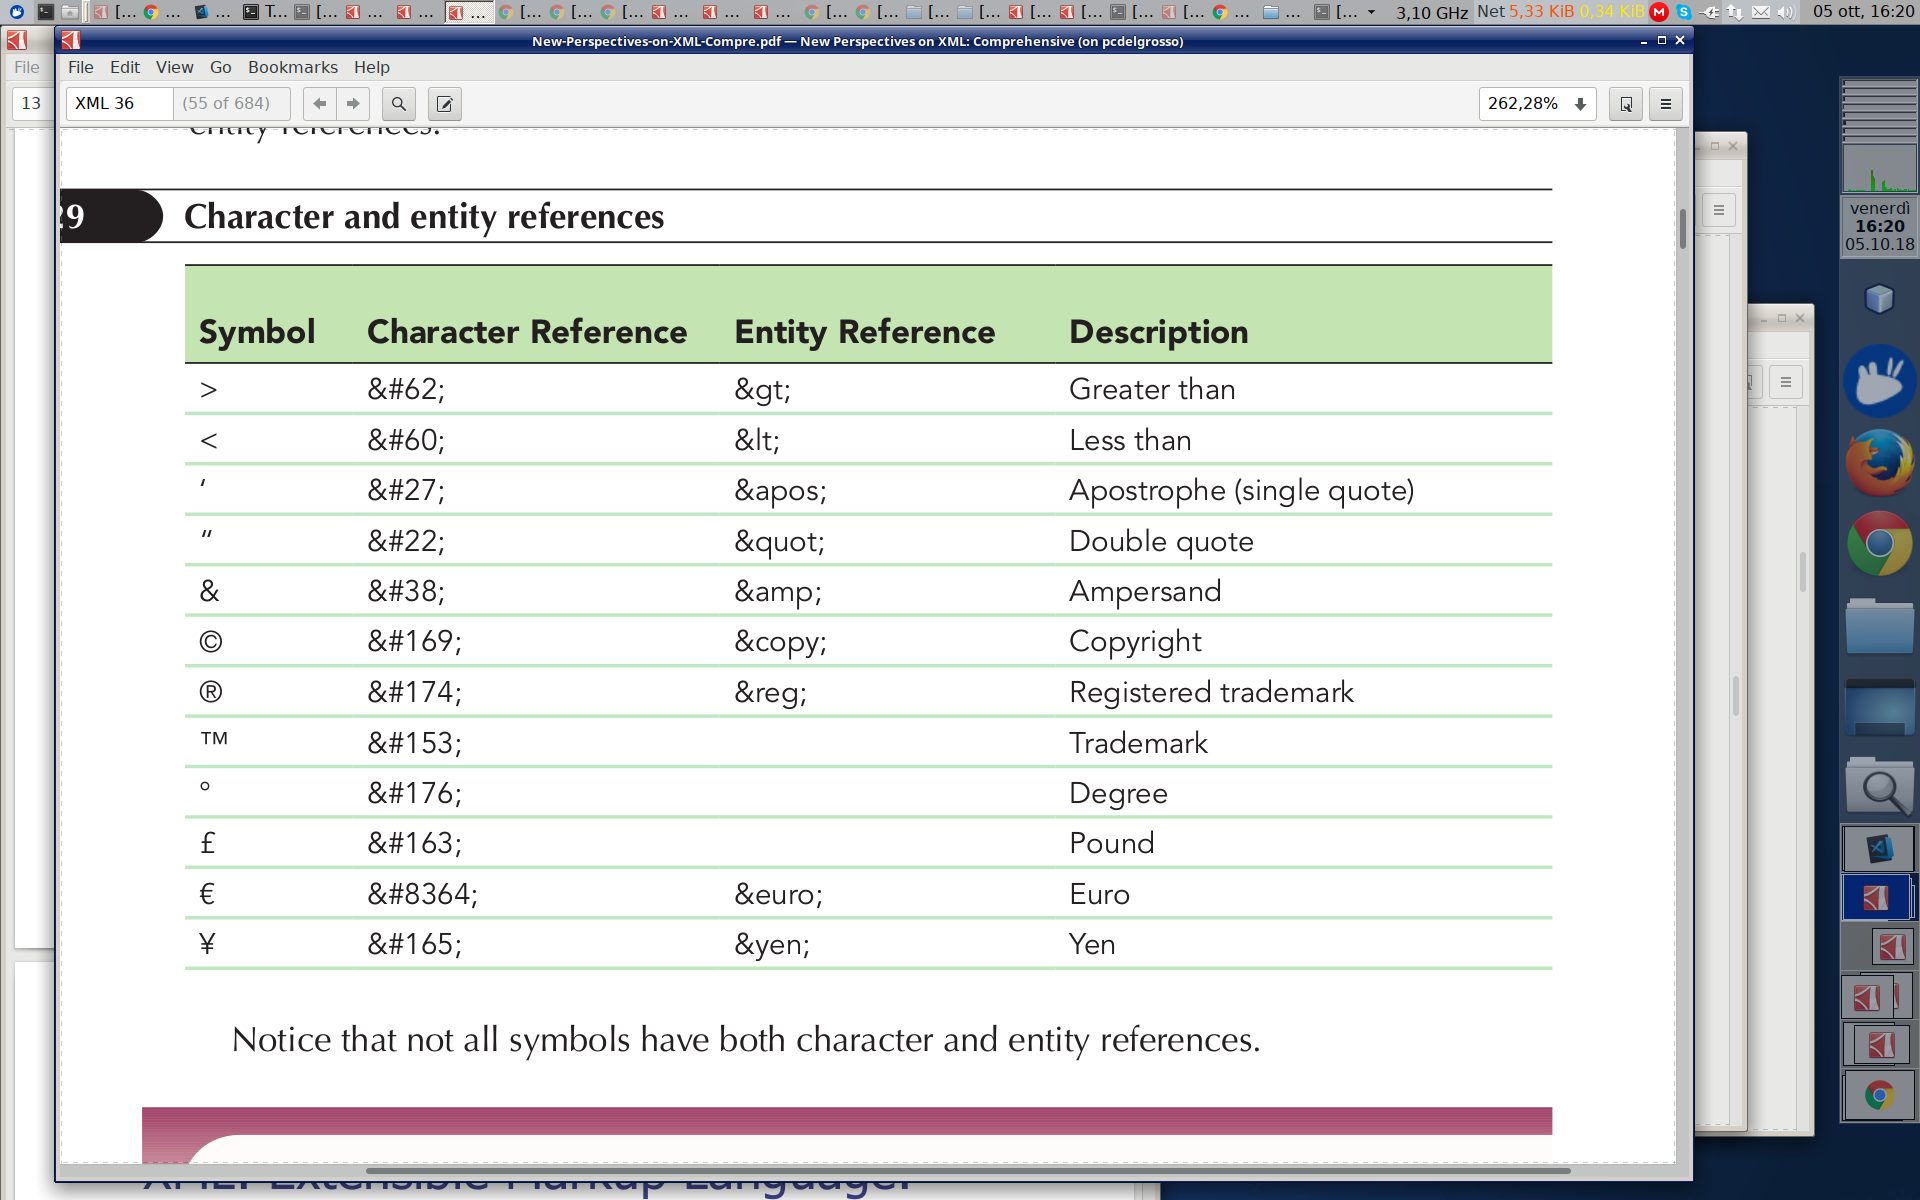
\includegraphics[width=0.95\textwidth]{imgs/xml-Character-Entity.png}
	\end{center}
\begin{tiny}\textit{immagine dal libro New Perspectives on XML, 3rd Edition}\end{tiny}
\end{frame}


\begin{frame}
    \frametitle{Fondamenti XML}
    \framesubtitle{eXtensible Markup Language}
    \addtocounter{nframe}{1}

	\begin{block}{Text Character Parsing}
		Il contenuto testuale di un elemento XML può essere diviso in tre categorie:
		parsed character data, character data, and white space.
	\end{block}

	\begin{block}{Text Character Parsing}
		\begin{itemize}
			\item \texttt{PCDATA}
			\item \texttt{CDATA}
			\item \texttt{White Space}
		\end{itemize}
	\end{block}

\end{frame}


\begin{frame}
    \frametitle{Fondamenti XML}
    \framesubtitle{eXtensible Markup Language}
    \addtocounter{nframe}{1}

	\begin{block}{Parsed Character Data}
		Parsed character data (PCDATA) si riferisce a tutti quei caratteri che XML tratta come parte del codice e quindi vengono interpretati dai parser.
	\end{block}

	\begin{block}{PCDATA}
		\begin{itemize}
			\item XML declaration
			\item Opening tag e  closing tag
			\item Character or entity references
			\item Commenti
		\end{itemize}
	\end{block}

\end{frame}

% The presence of PCDATA can cause unexpected errors to occur within a document
% This means that symbols such as \&, <, or >, which are all used in ­creating
% markup tags or entity references, are extracted and the appropriate content is used in your program.

\begin{frame}
    \frametitle{Fondamenti XML}
    \framesubtitle{eXtensible Markup Language}
    \addtocounter{nframe}{1}

	\begin{block}{Parsed Character Data}
		La presenza di contenuti di tipo PCDATA può causare errori inaspettati.
	\end{block}

	\begin{block}{XML PCDATA}
		Caratteri speciali che sono utilizzati dalla specifica XML come \texttt{\&, <, >} non possono essere utilizzati come contenuto testuale.
	\end{block}

\end{frame}


% Character Data

\begin{frame}
    \frametitle{Fondamenti XML}
    \framesubtitle{eXtensible Markup Language}
    \addtocounter{nframe}{1}

	\begin{block}{Character Data}
		I dati di tipo ``Character Data'' non vengono interpretati dal parser XML.
		\\ La sequenza di caratteri viene trattata come puro contenuto.
		\\In definitiva una sezione \textit{CDATA} è un blocco di testo.
	\end{block}

	\begin{block}{XML CDATA: sintassi}
		\begin{center}
			\texttt{
				 <![CDATA [
					 \\character data
					 \\]]>
			}
		\end{center}
	\end{block}

\end{frame}


%A CDATA section

\begin{frame}
    \frametitle{Fondamenti XML}
    \framesubtitle{eXtensible Markup Language}
    \addtocounter{nframe}{1}

	\begin{block}{Character Data}
		Le sezioni di testo CDATA possono essere inserite in qualsiasi parte del documento XML.
		\\ Utile per inserire una sezione di testo com molti caratteri speciali.
	\end{block}

\end{frame}

\begin{frame}
    \frametitle{Fondamenti XML}
    \framesubtitle{eXtensible Markup Language}
    \addtocounter{nframe}{1}

	\begin{block}{CDATA: qualche vincolo}
		\begin{itemize}
			\item Non è possibile inserire commenti in una sezione CDATA.
			\item Non è possibile annidare sezioni CDATA. 
			\item Non possono essere vuote.
			\item i simboli ``]]'' non sono ammessi.
		\end{itemize}
	\end{block}

\end{frame}


\begin{frame}
    \frametitle{Fondamenti XML}
    \framesubtitle{eXtensible Markup Language}
    \addtocounter{nframe}{1}

	\begin{block}{Esempio ed esercizio}
		Inserire all'interno di un tag un frammento di codice HTML
	\end{block}

	\begin{block}{CDATA: esempio}
		\begin{center}
			\texttt{
			<htmlCode>
			 <![CDATA[
			 		<h1>Capitolo Primo</h1>
			 		<h2>Sezione Seconda</h2>
			 	]]>
			 </htmlCode>
			 }
		\end{center}
	\end{block}

\end{frame}


% White Space

\begin{frame}
    \frametitle{Fondamenti XML}
    \framesubtitle{eXtensible Markup Language}
    \addtocounter{nframe}{1}

	\begin{block}{White Space: esempio}
		\begin{itemize}
			\item Gli spazi bianchi sono ignorati quando sono tra i tag.
			%White space is ignored when it is the only character data between element tags
			\item Gli spazi bianchi sono ignorati all'interno del prologo e dell'epilogo e all'interno dei tag. 
			%White% space is ignored within a document prolog and epilog, and within any element tags
			\item Gli spazi bianchi inseriti nel valore di un attributo sono trattati come parte del contenuto.
			%White space within an attribute value is treated as part of the attribute value
			\item Non vengono strippati gli spazi all'interno del contentuto testuale degli elementi.
			%no white space ­stripping occurs for element content, which means that the content of the XML element
		\end{itemize}
	\end{block}

	\begin{tiny}
		I white space sono caratteri non stampabili
	\end{tiny}


\end{frame}

% Inserting a Processing Instruction

\begin{frame}
    \frametitle{Fondamenti XML}
    \framesubtitle{eXtensible Markup Language}
    \addtocounter{nframe}{1}

	\begin{block}{Processing Instruction}
		Una \textit{processing instruction} è un comando, una direttiva, che indica al parser XML in che modo elaborare e trattare tutto o parte del documento XML.
	\end{block}

	\begin{block}{Processing Instruction: sintassi}
		\begin{center}
			\texttt{<?target instruction ?>}
			\\\texttt{<?xml-stylesheet type=”text/css” href=”main.css” media=”all” ?>}
		\end{center}
	\end{block}
\begin{tiny}
    \textit{Molteplici processing instruction possono co-esistere all'interno di un unico documento XML.}
\end{tiny}
    
	% Multiple processing instructions can exist within the same XML document for different
% media types

\end{frame}



\begin{frame}
    \frametitle{Fondamenti XML}
    \framesubtitle{eXtensible Markup Language}
    \addtocounter{nframe}{1}

	\begin{block}{Processing Instruction: sintassi}
		\begin{center}
			\texttt{<?target instruction ?>}
			\\\texttt{<?xml-stylesheet type=”text/css” href=”main.css” media=”all” ?>}
		\end{center}
	\end{block}


	\begin{block}{Processing Instruction}
		 \textbf{Target}: identifica il tool al quale la processing instruction è diretta.
		 \\\textbf{Instruction}: identifica le informazioni che il documento passa al parser per essere elaborate. Le istuzioni hanno la forma degli attributi (nome-valore).
	\end{block}

\end{frame}

% Working with Namespaces

% involves two steps:
% 1. Declare the namespace.
% 2. Identify the elements and attributes within the document that belong to that
% namespace.


\begin{frame}
    \frametitle{Fondamenti XML}
    \framesubtitle{eXtensible Markup Language}
    \addtocounter{nframe}{1}

	\begin{block}{Namespaces}
		Un namespace può essere visto come una collezione di elementi e attributi e un insieme di regole che ne determinano la struttura e il contenuto.
	\end{block}

	\begin{block}{Namespaces}
		\begin{center}
			\texttt{<element xmlns:prefix=”uri”> ... </element>}
			\\\texttt{<element xmlns=”uri”> ... </element>}
			\\\texttt{<tei:TEI xmlns:tei=``http://www.tei-c.org/ns/1.0''>}
			\\\texttt{<TEI xmlns=``http://www.tei-c.org/ns/1.0''>}
		\end{center}
	\end{block}

\end{frame}

% (URI)—a text string that uniquely identifies a resource.
% The purpose of a URI is simply to provide a
% unique string of characters that identify a resource.
% One version of a URI is the Uniform Resource Locator (URL)
% URLs serve as a built-in mechanism on the web for generating unique addresses
% Note that although a URI
% doesn’t actually need to point to a real site on the web, it’s often helpful to place
% documentation at the site identified by a URI so users can go there to learn more
% about the XML vocabulary being referenced.


% The number of namespace attributes that can be declared within an element is
% unlimited.

% root element so that each namespace is available to all
% elements within the document

% You can declare a default namespace by omitting the prefix in the namespace ­declaration.
% Any descendant element or attribute is then considered part of this namespace unless a
% different namespace is declared within one of the child elements.


\begin{frame}
    \frametitle{Fondamenti XML}
    \framesubtitle{eXtensible Markup Language}
    \addtocounter{nframe}{1}

	\begin{block}{Namespaces}
		Un namespace viene ereditato da tutti gli elementi discendenti dell'elemento in cui esso è stato dichiarato.
	\end{block}

	\begin{block}{Namespaces}
		Generalmente si dichiarano tutti i namespace nell'elemento root così da avere a disposizione tutti gli elementi dei vari namespace in tutto il documento XML
	\end{block}

\end{frame}

% esempio di dichiarazione di vari namespace in un documento XML

% Declaring a Namespace
% • To declare a namespace for an element within an XML document, add the
% xmlns:prefix attribute to the opening tag of the element using the syntax
% <element xmlns:prefix=”uri”> ... </element>
% where element is the element in which the namespace is declared, prefix is the
% namespace prefix, and uri is the URI of the namespace.
% • To declare a default namespace, add the xmlns attribute without specifying a prefix,
% as follows:
% <element xmlns=”uri”> ... </element>

% immagini di riepilogo












% Attributes can only store a value, while elements can also store child elements and attributes.
% An element can appear more than once within a parent node, but an attribute can appear only once. The order of attributes is not significant and there is no way to control the order of attributes in XSD. If the attribute is present the default value is not assigned, even if the value of the attribute is an empty string.
% the default value of elements is assigned only when the element is present and is empty
% Elements are mandatory by default while attributes are optional by default.


%Both HTML and XML use tags in similar ways, often creating distinctly hierarchical structures to present data to users.

% Like HTML documents, XML documents can be created and viewed with a basic text editor such as Notepad or TextEdit. More sophisticated XML editors are available, and using them can make it easier to design and test documents.




% tanti vocabolari XML
% Bioinformatic Sequence Markup
% Language (BSML) Coding of bioinformatic data
% Extensible Hypertext Markup Language
% (XHTML) HTML written as an XML application
% Mathematical Markup Language
% (MathML) Presentation and evaluation of mathematical equations
% and operations
% Music Markup Language (MML) Display and organization of music notation and lyrics
% Weather Observation Definition
% Format (OMF) Distribution of weather observation reports, forecasts, and
% advisories
% Really Simple Syndication (RSS) Distribution of news headlines and syndicated columns
% Synchronized Multimedia Integration
% Language (SMIL) Editing of interactive audiovisual presentations ­involving
% streaming audio, video, text, and any other media type
% Voice Extensible Markup Language
% (VoiceXML) Creation of audio dialogues that feature synthesized
% speech, digitized audio, and speech recognition
% Wireless Markup Language (WML) Coding of information for smaller-screened devices, such
% as PDAs and cell phones


\section{Validare XML }
%% 	    %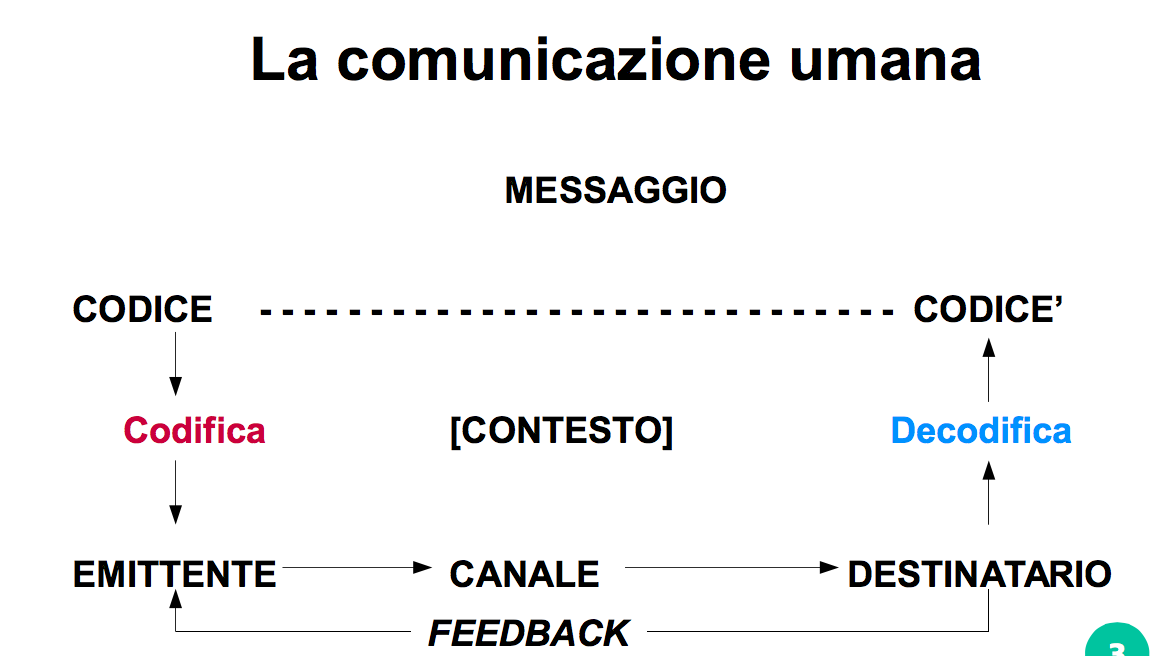
\includegraphics[width=.5\textwidth]{../imgs/comunicazioneUmana.png}




% L’applicazione di tecnologie informatiche nelle discipline umani- stiche, e in particolare nelle scienze letterarie, ha come suo fondamento la rappresentazione degli oggetti che costituiscono il loro dominio di studio. Tali oggetti sono in linea generale i testi.

% l’analisi del processo di scoperta e rappresentazione dell’oggetto testo e della sua struttura non può prescindere da una de- terminazione di cosa si intenda per testo, o quantomeno da una assun- zione implicita sulla sua natura;

% Il testo è un oggetto complesso in quanto è in grado di veicolare si- gnificato (e di rivestire dunque interesse scientifico) su più livelli strutturali, anche attraverso l’instaurazione di molteplici relazioni tra più livelli.

% Non possediamo nessuna teoria sufficientemente completa del testo

% Il fatto è che la rappresentazione (e a maggior ragione l’elaborazione) informatica è ontologicamente formale in senso stret- to.

% Il termine “testo”  si riferisce a un oggetto complesso e plurale, in cui esiste 
%- un livello materiale, il supporto e le tracce d’inchiostro, 
%- un livello astratto, la sequenza verbale, la quale a sua volta genera una serie di livelli di contenuti semantici.

% Lo studio del sapere ha come oggetto immediato i testi (letterari e non). Nella nostra cultura la quasi totalità dei testi letterari (fino a questo momento) è costituita da testi scritti su supporti cartacei di varia natura e forma.

% A questa struttura rigida del codice nell’ambito informatico (codice binario) va confrontata la complessa intersezione di codici che costituiscono un testo (da memorizzare).

% il termine “testo” non denota una entità acritica, oggetto della memorizzazione, affermando banalmente si tratta di una entità informativa complessa.

% Molteplici teorie del testo, quasi tutte sbilanciate sul livello verbale-semantico (linguistica testuale)

% Possiamo concludere che il testo è l’invariante, la successione di valori, rispetto alle variabili dei caratteri, della scrittura.
% Il testo è dunque una successione fissa di significati grafici (Segre, 1985).

% il testo come una entità astratta invariante, che in ogni operazione di realizzazione materiale della sequenza di simboli grafici determina la struttura fisica di un og- getto sensibilmente concreto (ovvero capace di attivare uno dei canali recettivi dell’uomo verso stimoli esterni), che costituisce il supporto materiale, stabile e riproducibile dell’informazione testuale. Distin- gueremo questo oggetto dal testo chiamandolo documento.

% Testo vs Documento

% oltre alla sequenza di grafemi, a un testo nel senso da noi indicato possono essere ascritte anche le segmentazioni logiche e le partizioni interne di interi blocchi
% il testo ha una certa struttura, i cui elementi sono determinati dalla struttura logico semantica del discorso,

% esiste anche un modello documento
% possibilità significative che derivano da una semantizzazione esplicita degli elementi non verbali di un testo scritto.
% ruolo della disposizione tipografica e topografica del segno grafico nella pagina bianca

% quale concezione o modello ontologico del testo è implicata nella rappresentazione informatica?

% natura del testo: il testo è, in un senso importante, una “ordered hierarchy of content objects (OHCO)”, una gerarchia ordinata di oggetti di contenuto [DeRose et al., 1990:3]. Gli oggetti di contenuto testuale a cui si fa riferimento in questa teoria sono sostanzialmente le strutture editoriali astratte di cui si com- pone un testo. Essi sono gerarchici poiché alcuni degli oggetti testuali con- tengono altri, e ordinati in quanto esiste una relazione lineare tra due oggetti posti sul medesimo livello gerarchico.

% il genere determina gli elementi che costituiscono il testo, quindi il tipo di documento. Reciprocamente un genere testuale è individuato dalla classe di oggetti di contenuto che contiene.
% Su questo impianto teorico si è basata, ad esempio, la prima fase del lavoro della Text Encoding Initiative.
% Sono però stati riscontrati una serie di problemi di rappresentazione che costituiscono dei veri e propri controesempi. Ci sono moltissimi casi in cui non esiste assolutamente accordo tra gli specialisti dei testi nell’asserire l’appartenenza di un dato testo a un tipo piuttosto che a un altro.  Questi diversi insiemi di elementi di contenuto non possono essere ricondotti a una struttura gerarchica unitaria.

% classi di elementi testuali che si sovrappongono rompendo i confini della struttura gerarchica di un documento: esempio: struttura metrica e quella morfosintattica di un testo poetico.. (Esempio clavius righe e sentence). Questi elementi si comportano come se appartenessero a diverse gerarchie di oggetti testuali che si sovrappongo.
% Prospettiva analitica:  “ogni prospettiva analitica su un testo determina una struttura gerarchica di oggetti di contenuto”.
% Un corollario operativo di questa tesi è che se due elementi a e b si sovrappongono, allora essi appartengono a due diverse prospettive analitiche.

% Ma è vero che a ogni coppia di elementi che si sovrappongono cor- rispondono due distinte prospettive teoriche? occorrenza di alcuni oggetti testuali che, pur appartenendo ragionevolmente a una medesima pro- spettiva analitica si sovrappongono.
%Se due oggetti testuali evidenziati da una prospettiva teorica si sovrap- pongono, allora essi appartengono rispettivamente a due sottoprospet- tive diverse della prospettiva teorica principale. Questa ultima revisione della teoria gerarchica abbandona qualsiasi assunto di tipo essenzialista. In questa ottica il testo diventa un sistema a più livelli, che corrispondono a diversi punti di vista dell’osservatore.
% • il testo è un oggetto reale dotato di una sua struttura che corrisponde alla struttura del linguaggio di rappresentazione;
% • la struttura o meglio le strutture del testo sono strutture gerar- chiche: le sottoprospettive, comunque esse siano definite, dan- no luogo a gerarchie.

% Alcune teorie avanzano la necessità di abbandonare l’assunto ontologico che il testo sia un oggetto reale del mondo, dotato di una struttura intrinseca: Il testo è dunque una entità che viene costruita e non scoperta e a- nalizzata dalla attività scientifica. soluzione interessante e intellettualmente stimolante alle aporie determinate dal- la teoria gerarchica del testo, specialmente nella tematizzazione del ruolo dell’osservatore nei processi di rappresentazione.

% cos'è il testo (uso comune):
%a) un documento materiale composto da fogli di carta rilegati (o spillati o semplicemente raccolti insieme da un nastro di carta) che contengono tracce di inchiostro variamente disposte (oltre a eventuali tracce di altri materiali)
%b) un discorso linguistico fissato tramite la scrittura su un docu- mento materiale
%c) un’opera dell’ingegno che viene costituita da quel discorso

% cos'è un testo (uso più specialistico)
% d) lo stato linguistico di un singolo testimone materiale di un’opera
% e) lo stato linguistico di un medesimo testimone di un’opera che presenta diverse lezioni identificabili
% f) una versione edita di un’opera
% g) una sequenza coerente di enunciati in una lingua naturale
% Teso è l'invariante rispetto ai segni, è la succesione di valori invariabili. Il testo, dunque è ciò che permane, l’invariante, in ogni operazione di riproduzione materiale della sequenza di simboli grafici.
% Questa definizione di testo come un oggetto astratto allografico sembra fornire un criterio di individuazione di un testo in base al prin- cipio di identità per sostituzione

%OHCO: alla do- manda che cosa è un testo veramente rispondiamo che un testo è un oggetto linguistico astratto organizzato secondo una struttura gerar- chica ordinata di oggetti di contenuto. (Asserzione poi rilevatasi fallace). Ma l’idea di una preminenza della struttura gerarchica nella testualità ha mantenuto un ruolo descrittivo ed esplicativo essenziale.

\section{Document Typed Definition - DTD}
%% Vedere Slide CHiara. Roberto
% Portabilità e riutilizzabilità
% schema di codifica
% TEI XML focuses on the meaning of text, rather than its appearance.

\begin{frame}
	\frametitle{Importanza della codifica digitale}
	\framesubtitle{Perché effettuare la codifica}
	\addtocounter{nframe}{1}

	\begin{block}{Digitalizzare un testo}
		Digitalizzare per poter favorire l'elaborazione e il trattamento automatico dei testi
	\end{block}

	\begin{block}{Trattamento dei testi}
        \begin{itemize}
            \item  analisi di tipo linguistico (linguistica computazionale,
            database testuali, corpora linguistics)
            \item analisi di altro tipo (metrica, stilistica, etc.)
            \item ricerca testuale avanzata
            \item pubblicazione in vari formati (sul web, come ebook, a
            stampa)
            \item didattica
        \end{itemize}
 
    \end{block}
\end{frame}

\begin{frame}
	\frametitle{Importanza della codifica digitale}
	\framesubtitle{Perché effettuare la codifica}
	\addtocounter{nframe}{1}

	\begin{block}{Digitalizzare un testo}
		Per facilitare e garantire una universalità di accesso al loro contenuto 
	\end{block}

	\begin{block}{Vantaggi della digitalizzazione}
        \begin{itemize}
            \item Edizioni elettroniche garantiscono diffusione capillare
            (via web) e nuove funzionalità (ipertesti, ricerca, etc.)
            \item Permettono anche di preservare i documenti più antichi
            (e fragili) riducendone la consultazione diretta
        \end{itemize}
     \end{block}
\end{frame}

\begin{frame}
	\frametitle{Importanza della codifica digitale}
	\framesubtitle{Perché effettuare la codifica}
	\addtocounter{nframe}{1}

	\begin{block}{Superare i problemi dei documenti digitali}
		\begin{itemize}
            \item disponibilità di hardware e software
            \item sistemi proprietari chiusi
            \item elevata obsolescenza e limitata manutenibilità
            \item difficile portabilità su piattaforme diverse
        \end{itemize}
	\end{block}
	
\end{frame}

\begin{frame}
	\frametitle{Importanza della codifica digitale}
	\framesubtitle{Perché effettuare la codifica}
	\addtocounter{nframe}{1}

	\begin{block}{Sistemi non adatti}
		\begin{itemize}
            \item word processing: WYSIWYG (What You See Is What You Get)
            \item sistemi proprietari chiusi (Word, Adobe, etc)
            \item elevata obsolescenza e limitata manutenibilità
            \item difficile portabilità su piattaforme diverse (windows, linux)
        \end{itemize}
	\end{block}
	
\end{frame}

\begin{frame}
	\frametitle{Importanza della codifica digitale}
	\framesubtitle{Perché effettuare la codifica}
	\addtocounter{nframe}{1}

	\begin{block}{Massimizzare le seguenti proprietà: Portabilità}
		\begin{itemize}
            \item indipendenza dall’hardware: processore, supporto, output
            \item indipendenza dal software: sistemi operativi, applicazioni di authoring, applicazioni di visualizzazione
            \item indipendenza dai sistemi di codifica dei caratteri
            \item indipendenza logica: da un particolare processo applicativo
        \end{itemize}
	\end{block}
	
\end{frame}




%La codifica dell’informazione gode delle seguenti proprietà:
% indipendenza dall’hardware, ovvero da una particolare architettura elaborativa (processore), da un particolare supporto digitale (disco magnetico, disco ottico, etc.), o da un particolare dispositivo o sistema di output (video, stampa);
% indipendenza dal software, sia sistemi operativi, sia applicazioni deputate alla creazione, analisi, manipolazione e visualizzazione di testi elettronici; (formati di dati proprietari mutamente incompatibili)
% indipendenza logica dalle applicazioni ovvero indipendenza semantica dello schema di codifica da un particolare processo applicativo.

% L’archiviazione su supporto digitale del patrimonio letterario e culturale delle culture mondiali deve misurarsi con questi problemi, e adottare degli schemi di codifica capaci di garantire la massima portabilità. 



% Una risorsa informativa digitale è portabile se è intercambiabile tra sistemi diversi, riutilizzabile in molteplici processi computazionali anche a distanza di tempo, e integrabile da ulteriori risorse informative omogenee


%  Esso deve divenire uno standard
% I vantaggi di uno standard formale o informale, oltre alla portabilità sta anche nella sua apertura, ovvero nella disponibilità pubblica delle sue specifiche.



% La disposizione alla rappresentazione di strutture astratte non pone limiti alla natura e tipologia delle caratteristiche testuali che si possono codificare in un testo elettronico. Queste possono essere utilizzate indifferentemente 

% Se il linguaggio è dotato di una sintassi che permette di specificare le relazioni tra gli elementi, essa può essere usata per rappresentare la struttura e l’organizzazione del testo a un determinato livello di descrizione, o i rapporti tra elementi appartenenti a diversi livelli.


% un sistema di codifica dichiarativa assiste un autore nel processo di scrittura, poiché focalizza l’attenzione sul contenuto di un testo (o sulla struttura del contenuto) piuttosto che sulla sua forma grafica.

% I sistemi di markup dichiarativo introducono consistenti vantaggi anche nei processi produttivi editoriali e nella gestione dei flussi informativi aziendali. Poiché un medesimo schema di codifica dichiarativo può essere utilizzato in molteplici forme di trattamento informatico, i costi di produzione e gestione di una base dati testuale vengono fortemente ridotti.

% I sistemi di codifica dichiarativa peraltro si prestano ottimamente per rappresentare strutture complesse come riferimenti incrociati e collegamenti tra elementi all’interno di un testo, ma anche tra più testi

% Infatti un database offre dei notevoli vantaggi dal punto di vista delle prestazioni computazionali e della velocità di ricerca, anche se richiede in generale una ingente quantità di memoria per l’archiviazione.

% La codifica permette allo studioso di esplicitare le sue ipotesi interpretative.

% OHCO: efficienza computazionale che la struttura gerarchica mostra; 

% I linguaggi di markup dichiarativi permettono di predicare l’appartenenza di un dato segmento testuale a una classe di strutture testuali definita dall’utente;
%  Così è possibile descrivere formalmente le caratteristiche di un testo in modo indipendente da particolari finalità di trattamento
% da contingenti forme di presentazione grafica su un qualsivoglia supporto fisico

% I linguaggi di markup dichiarativi, e in particolare SGML e XML, si sono rivelati dei veri e propri strumenti di supporto all’analisi computazionale dei testi
% la sintassi del linguaggio di codifica può essere usata per rappresentare le relazioni tra gli elementi strutturali di un testo, a un determinato livello di descrizione.



%\section{Linguaggi di marcatura}
%% intro linguaggi di Markup

% La rappresentazione che vogliamo eseguire deve essere eseguira mediante le istruzioni, le convenzioni e i costrutti  messi a disposizione da un opportuno linguaggio che sarà definito formalmente da una specifica sintassi e da una precisa semantica.
% linguaggio in cui tutti i termini sono definiti esplicitamente e usati in modo conforme a tali definizioni.

% Si deve notare che «ogni dato su cui l’elaboratore deve operare viene rappresentato a livello elementare mediante una sequenza (o stringa) di simboli


% In modo parallelo ai linguaggi di programmazione, anche i linguaggi di markup possono essere divisi in due tipologie: linguaggi procedurali, che nella letteratura vengono indicati anche come specific markup language; e linguaggi dichiarativi o descrittivi, detti anche generic markup language.

% I sistemi di codifica procedurale sono per definizione orientati a una singola applicazione. la portabilità di un testo codificato con sistemi procedurali è molto limitata.


% nei linguaggi di markup dichiarativi/descrittivi invece di specificare quali operazioni di formattazione vanno effettuate in un particolare punto del testo, si dichiara che un dato segmento testuale è istanza di un tipo di struttura editoriale del testo; insomma, si dichiara: “questo è un titolo”


% Un sistema di codifica dichiarativo dunque è orientato alla rappresentazione delle caratteristiche o elementi che costituiscono un testo, indipendentemente dalle finalità specifiche per le quali il testo è stato memorizzato e codificato.

% Tra questi hanno una notevole importanza ai fini della modellizzazione di testi, quei sistemi basati sui cosiddetti markup language.

% Il termine inglese markup designava nella stampa tipografica tutte le indicazioni e annotazioni simboliche aggiunte dall’autore o dall’editore su un manoscritto o su un dattiloscritto per istruire il tipografo

% Similmente un markup language è costituito da un set di istruzioni di un vero e proprio linguaggio orientato alla descrizioni dei fenomeni di composizione e struttura del testo.

% i linguaggi di markup infatti, consistono di un insieme di simboli che vengono inseriti all’interno o accanto al testo verbale.

% Un linguaggio di Markup, quindi, è un formalismo artificiale con il quale poter esprimente la rappresentazione o il modello del testo considerato.
% Un linguaggio (formale) sull'alfabeto A non è altro che un sottoinsieme di A*. Una grammatica formale serve proprio a definire un certo sottoinsieme di stringhe tra tutte quelle possibili su un dato alfabeto.



%Come i linguaggi procedurali, anche quelli dichiarativi vengono utilizzati inserendo all’interno del file di testo sequenze di caratteri. generalmente dette tag (etichette o marche)

%Più precisamente uno schema di codifica associa un insieme di caratteristiche o elementi costituenti di un oggetto testuale a un insieme di simboli, e le relazioni tra gli elementi testuali a relazioni sintattiche tra i simboli.
%% Un esempio (per esempio capitolo-titolo-paragrafo)..

\section{XML Schema Definition - XSD}
%% l’applicazione di metodologie computazionali nell’ambito della ricerca umanistica comporta due tipi, o meglio due fasi di formalizzazione:
% definizione e implementazione di strutture dati adeguate alla cattura dei fenomeni di interesse dell’umanista, e in particolare alla rappresentazione formale dei testi;
% specificazione di algoritmi che, applicati alle strutture dati, siano in grado di simulare i processi di manipolazione dei testi tipici della ricerca umanistica o in generale delle pratiche sociali che hanno a che fare in vario modo con i testi.

%% lo schema di codifica TEI impone al responsabile della codifica di effettuare delle scelte teoriche e interpretative che non sono pertinenti alla sua opera di semplice trascrittore.

%  uno di carattere epistemologico, riguarda la natura della codifica come processo di rappresentazione.
% carattere ontologico, e concerne il concetto generale di testo che «emerge» dalle teorie dei sistemi di codifica.

% domanda: codifica è un processo interpretativo oppure un processo riproduttivo?
%% lo schema di codifica TEI impone al responsabile della codifica di effettuare delle scelte teoriche e interpretative che non sono pertinenti alla sua opera di semplice trascrittore.


% la rappresentazione informatica è un processo semiotico: Ogni atto rappresentazionale o semiotico implica dei processi interpretativi 

% indagare più a fondo la natura della codifica e dell’idea di testo che la codifica presuppone.


% Naturalmente questo è possibile se tale descrizione del supporto fisico di un testo è riducibile a un struttura gerarchica.

% I problemi e le difficoltà determinati dagli schemi SGML per una codifica presentazionale in effetti, sono determinati proprio da questa metastruttura

% problema: utilizzazione dei simboli del linguaggio informatico in funzione di representare dei caratteri alfanumerici del testo

\begin{frame}
	\frametitle{Approfondimenti e Conclusioni}
	\framesubtitle{per comprendere la codifica}
	\addtocounter{nframe}{1}

	\begin{block}{Codifica del testo}
		L’applicazione di metodologie computazionali nell’ambito della ricerca umanistica comporta due aspetti di formalizzazione
	\end{block}

	\begin{block}{Due elementi}
		Formalizzazione dei dati e formalizzazione dell'elaborazione
	\end{block}

\end{frame}

\begin{frame}
	\frametitle{Approfondimenti e Conclusioni}
	\framesubtitle{per comprendere la codifica}
	\addtocounter{nframe}{1}

	\begin{block}{Formalizzazione dei dati}
		Definizione e implementazione di strutture dati adeguate alla cattura dei fenomeni di interesse dell’umanista, e in particolare alla rappresentazione formale dei testi;
	\end{block}

	\begin{block}{Formalizzazione dell'elaborazione}
		specificazione di algoritmi che, applicati alle strutture dati, siano in grado di simulare i processi di manipolazione dei testi tipici della ricerca umanistica o in generale delle pratiche sociali che hanno a che fare in vario modo con i testi.
	\end{block}

\end{frame}


\begin{frame}
	\frametitle{Approfondimenti e Conclusioni}
	\framesubtitle{per comprendere la codifica}
	\addtocounter{nframe}{1}

	\begin{block}{Codifica del testo}
		Il problema della codifica testuale rientra in generale nel primo tipo di formalizzazione (Dati).
	\end{block}

\end{frame}

\begin{frame}
	\frametitle{Approfondimenti e Conclusioni}
	\framesubtitle{per comprendere la codifica}
	\addtocounter{nframe}{1}

	\begin{block}{problemi teorici}
		La codifica è un processo assai più complesso delle semplice e meccanica correlazione biunivoca di strutture rappresentazionali.
	\end{block}

\end{frame}

\begin{frame}
	\frametitle{Approfondimenti e Conclusioni}
	\framesubtitle{per comprendere la codifica}
	\addtocounter{nframe}{1}

	\begin{block}{problema del testo}
		la specificazione di cosa sia un testo e di quale legame sussista tra questa specificazione, i processi dell’interpretazione e i linguaggi formali con i quali essa viene descritta.
	\end{block}

\end{frame}

\begin{frame}
	\frametitle{Approfondimenti e Conclusioni}
	\framesubtitle{per comprendere la codifica}
	\addtocounter{nframe}{1}

	\begin{block}{Norme TEI}
		Le linee guida di codifica TEI impongono a chi codifica di effettuare delle scelte teoriche e interpretative che non sono imputabili alla semplice trascrizione.
    \end{block}
    
    \begin{block}{Processo di codifica}
        La codifica è un processo interpretativo non solo un processo riproduttivo.
        \\Non è quindi un semplice processo di trascrizione!
    \end{block}
    

\end{frame}


\begin{frame}
	\frametitle{Approfondimenti e Conclusioni}
	\framesubtitle{per comprendere la codifica}
	\addtocounter{nframe}{1}

	\begin{block}{Codifica come interpretazione}
		Conseguentemente ogni processo di codifica (inclusi quelli di codifica informatica del testo) è il risultato di una interpretazione.
    \end{block}
    
    \begin{block}{Rappresentazione e interpretazione}
        In ogni caso non esiste nessun genere di rappresentazione di un testo che si possa definire libera da processi interpretativi.
    \end{block}

\end{frame}

\begin{frame}
	\frametitle{Approfondimenti e Conclusioni}
	\framesubtitle{per comprendere la codifica}
	\addtocounter{nframe}{1}

	\begin{block}{Esempio}
		L’assunzione che una data traccia grafica ``A'' sia una istanza di un data classe astratta di tracce che identifichiamo come il carattere ``a''. Richiesti molti sforzi interpretativi.
    \end{block}
    
    \begin{block}{Rappresentazione e interpretazione}
        In linea di principio non è sempre possibile dire in modo non ambiguo che una traccia su un supporto fisico appartiene a una certa classe di iscrizioni che chiamiamo carattere.
    \end{block}

\end{frame}


\begin{frame}
	\frametitle{Approfondimenti e Conclusioni}
	\framesubtitle{per comprendere la codifica}
	\addtocounter{nframe}{1}

	\begin{block}{Certezza e soggettività}
		\textbf{Ogni interpretazione può godere di diversi gradi di certezza e di soggettività. In ogni caso non esiste nessun genere di rappresentazione di un testo che si possa definire libera da processi interpretativi.}
    \end{block}
   
\end{frame}

\begin{frame}
	\frametitle{Approfondimenti e Conclusioni}
	\framesubtitle{per comprendere la codifica}
	\addtocounter{nframe}{1}

	\begin{block}{Linguaggio teorico}
		Lo schema di codifica è un linguaggio teorico usato per costruire teorie o modelli di fenomeni testuali
    \end{block}

    \begin{block}{Linguaggio teorico}
        La stessa costruzione di un linguaggio teorico riflette un determinato modello del mondo (soggettivo o condiviso).
        \\ \textit{si presuppone una teoria ontologica del testo}.
    \end{block}
   
\end{frame}

\begin{frame}
	\frametitle{Approfondimenti e Conclusioni}
	\framesubtitle{per comprendere la codifica}
	\addtocounter{nframe}{1}

	\begin{block}{Obiettivo}
		\begin{itemize}
			\item Sviluppare teorie e modelli formali del testo (o di alcuni suoi livelli descrittivi)
			\item Individuare formalismi atti a esprimerli in modo computazionalmente accettabile
		\end{itemize}
	
    \end{block}
   
\end{frame}



% OHCO: La ragione di tanto attaccamento all’idea di struttura gerarchica ovviamente non è immotivata. Il fatto è che XML (e SGML) può essere considerato sia un formalismo sia un modello di dati espresso da quel formalismo, e tale (meta)modello è appunto un albero ordinato etichettato.

% Il prezzo costituito dall’adozione di un modello di dati così vincolante, d’altra parte, paga il vantaggio di potere validare in modo automatico ogni istanza di dati rispetto al modello mediante algoritmi generali ben conosciuti e computazionalmente trattabili, ciò che a sua volta consente di costruire sistemi di elaborazione degli stessi dati consistenti ed efficaci (al netto dei costrutti ID/IDREF).

% Le manifestazioni di queste difficoltà sono state comunemente rubricate come il problema delle gerarchie sovrapposte (overlapping hierarchies)
% In termini semplici il problema OH dal punto di vista sintattico consiste nel fatto che, dati due oggetti logici presenti in un testo, le coppie di tag bilanciati che li rappresentano non si annidano propriamente ma si sovrappongono.
%Tale situazione è sintatticamente e semanticamente vietata in XML

% ipotetiche soluzioni
% Non è un caso che negli ultimi dieci anni, proprio in parallelo con l’inarrestabile diffusione di XML nel mondo dell’elaborazione testuale (e non solo) e della TEI nella comunità umanistica si sono moltiplicati i tentativi di trovare delle soluzioni definitive al problema.
% soluzioni interne e soluzioni esterne al paradigma XML. Per questo alla completezza e congruenza va affiancata una serie di ulteriori criteri valutativi di natura teorica, tecnica e pragmatica

% In generale tutte le soluzioni proposte finora hanno grossi limiti per quel che concerne la facilità di gestione e manutenzione

% La visione pluralista del testo portata alle sue estreme conseguenze, eccede i limiti sintattici di un formalismo di codifica come XML. Lo standard, infatti, non è dotato di costrutti sintattici adeguati alla rappresentazione di molteplici sottoprospettive gerarchiche concorrenti che si sovrappongono ma che possono anche collegarsi e interrelarsi.

% Ogni modello descrive le caratteristiche del testo a un determinato livello, in base al punto di vista dell’osservatore, ma non coincide con esse.

% esempio con codice XML e grafico/immagine








% problema della complessità testuale
%% Se esistono proprietà dei testi irriducibili a qualsiasi formalizzazione anche minimale, allora queste non possono per definizione essere rappresentate e trattate con metodi computazionali.
% nella categoria delle gerarchie sovrapposte si possono distinguere diversi sottoproblemi di complessità crescente
% distinguere una “gerarchia delle gerarchie sovrapposte”.
% 1. Il caso più semplice e comune è quello della compresenza di due o più strutture (livelli) gerarchiche i cui elementi si sovrappongono.
% 2. concettualmente più complicato è quello di un elemento appartenente a una gerarchia che si estende oltre i confini dell’elemento in cui inizia o persino di uno dei suoi predecessori
% 3. Tecnicamente simile ma concettualmente distinto il caso di elementi composti da segmenti discontinui e non contigui 
% 4. Infine il caso più complesso che si verifica quando un dato elemento può auto-sovrapporsi illimitatamente.


% Leggibilità e facilità di comprensione da parte di un utente umano (sono esclusi dunque tutti i formati binari)
% Facilità di manutenzione e modifica
% Disponibilità di implementazioni software
% Compatibilità sintattica con XML
% Facilità di validazione (eventualmente sopravanzando le capacità di validazione di un parser XML standard)
% Possibilità di validazione incrociata tra gerarchie diverse Possibilità di formattazione ed elaborazione grafica e presentazionale
% Possibilità di estrapolare molteplici viste basate su uno o più tra le gerarchie presenti
% Possibilità di estrapolare sottoinsiemi gerarchici delle caratteri- stiche testuali
% Continuità del contenuto testuale serializzato

% Soluzioni interne al paradigma XML rientrano artifici sintattici che mantengono la conformità a XML
% XML come puro formalismo di serializzazione per modelli di dati non gerarchici
% Segmentazione: Un elemento logico che si sovrappone ai confini di un’altro (o di più altri) viene diviso in due (o n) elementi XML dello stesso tipo correlati mediante apposti attributi.
% Questa soluzione permetterebbe di risolvere sovrapposizioni di tipo (1) , (2) e (3), e può essere parzialmente validata mediante un oculato uso di attributi ID/IDREF.
% Elementi di congiunzione: Consiste nell’introduzione di un elemento XML (elemento di congiunzione) con la funzione metatestuale di esprimere l’unità logica di un fenomeno testuale rappresentato da più elementi XML distinti. Questa tecnica consente di trattare in linea teorica ogni caso di sovrapposizione e di non contiguità, di ordinamento inverso e di relazione n-aria tra oggetti testuali. Questo ultimo problema può essere risolto parzialmente adottando gli schemi di puntamento basati su range di caratteri previsto nello standard XPointer ma in questo caso l’elaborazione dei riferimenti richiederebbe l’uso di software ad hoc.
% Markup esterno (stand-off markup): Le tecniche basate su markup esterno sono di fatto identiche a quelle basate su elementi join. La differenza consiste nel fatto che in questo caso gli elementi che esprimono il collegamento di segmenti testuali nel documento XML base sono in un documento XML esterno. Il fatto di poter collocare i collegamenti in un documento autonomo consente di adottare un linguaggio XML per descrivere una struttura principale del documento base e uno diverso per la rappresentazione dei livelli di descrizione ulteriori.

% Ad esempio si può usare la TEI per la codifica del documento e XTM (XML Topic Maps) o RDF per esprimere le relazioni tra gli oggetti testuali. (interessante). Questa tecnica ha il vantaggio di poter disporre di modelli di dati e di sistemi di elaborazione complessi.

% Elementi Milestone: Un elemento milestone è un elemento XML vuoto che segnala un punto monodimensionale in un documento XML. si possono collocare liberamente sintatticamente in un documento XML. Questa strategia è ampiamente utilizzata nella TEI per veicolare le indicazioni sulla messa in pagina di un testo nel documento fonte da cui è stato memorizzato. Gli elementi milestone possono essere usati in coppie virtuali per segnalare i confini di segmenti arbitrari di testo che si sovrappongono agli elementi standard. Insieme a elementi di congiunzione o stand-off markup possono rappresentare virtualmente ogni genere di sovrapposizione, auto-sovrapposizione e segmentazione non contigua. 

%Gli elementi milestone offrono la massima flessibilità sintattica senza costringere a separare markup e contenuto. un parser XML può validare la corretta collocazione di un elemento vuoto rispetto a un modello di contenuto, o verificare che due elementi vuoti siano stati correlati mediante coppie di ID/IDREF. ma non può in alcun modo attribuire funzione strutturale alla sequenza di caratteri contenuta tra due elementi vuoti. non è accessibile come tale a una applicazione XML standard.



% Per questo negli ultimi anni la ricerca teorica sullo sviluppo di si- stemi di markup non gerarchici ha avuto un notevole stimolo

% L’ostacolo maggiore consiste nella individuazione di un modello di dati e di un formalismo a esso associato che possa essere validato ed elaborato mediante algoritmi generali e computazionalmente trattabili come avviene per il modello ad albero di XML.
%% rappresentazione di alberi concorrenti in un medesimo documento XML (Xconcur, JIITs)
%% In LMNL la soluzione del problema OH viene trovata uscendo definitivamente fuori dal paradigma gerarchico di XML
%% TexMECS e GODDAD: Markup Languages for Complex Documents. una notazione non molto dissimile da XML (provvede infatti anche strutture come gli attributi) la quale tuttavia permette di esprimere facilmente strutture sovrapposte, auto- sovrapposte e non contigue. In linea teorica questo grafo può esprimere tutte le possibili relazioni tra oggetti testuali linearizzati sottoforma di stringhe di caratteri etichettate mediante markup, inclusi i più complessi casi di auto- sovrapposizione o di frammentazione non contigua e non linearmente ordinata. 



% non possiamo dire apriori che uno schema di codifica testuale coglie l’essenza del testo più e meglio di un altro in base a un qualche assunto metafisico. Ma neppure si può affermare che ogni rappresentazione è vera in quanto costituisce il suo oggetto testo secondo esigenze specifiche e locali.

%% l’applicazione di procedure informatiche al trattamento dei testi richiede anche la simulazione dei processi che su di essi vengono effettuati.
% scrittura (il momento in cui il testo ha origine), edizione, lettura, analisi, interpretazione, archiviazione, catalogazione.

% Alcune caratteristiche sono comuni a tutti o a molti di questi tipi di testi, mentre altre sono assolutamente specifiche.

% In conclusione secondo la teoria OHCO un testo è una struttura gerarchica di oggetti logici, e la codifica non fa altro che esplicitare questa sua struttura essenziale.

% Ci accorgiamo dunque che la pratica comune nelle discipline che stu- diano i testi è quella di definire il loro oggetto a partire da un punto di vista interno alla disciplina stessa. Ciò dà luogo alla individuazione di diversi unità o elementi di conte- nuto testuale.

% TEI ha una struttura modulare, in cui ogni modulo corrisponde alla rappresentazione di un determinato punto di vi- sta metodologico sul testo.

% L’impianto finale dello schema di codifica della Text Encoding Initiative ha accolto in parte la nozione di sottoprospettiva ed ha svi- luppato una serie di costrutti sintattici e semantici in grado di rappre- sentare adeguatamente fenomeni di sovrapposizione e di parallelismo tra elementi testuali in XML.

% Una rappresentazione codificata di un testo dunque è «vera» se è internamente coerente, accettabile razionalmente nell’ambito di una teoria, in grado di rappresentare i fenomeni testuali rilevanti nel conte- sto di quella teoria o prospettiva metodologica, ed eventualmente di rendere conto dei rapporti tra strutture e fenomeni emergenti da rap- presentazioni (punti di vista) diverse.

% Il trasferimento del testo su supporto informatico propone allo studioso una serie di quesiti teorici (oltre a numerosi problemi pratici) a partire dal momento della decisione su quale particolare oggetto del mondo sia da considerare come “fonte” della memorizzazione.

% E come rileva lo stesso Dennet, possiamo benissimo sbagliarci nell’interpretare.

% La codifica elettronica di un testo, in quanto rappresentazione di un testo e delle sue caratteristiche median- te un linguaggio formale, si colloca interamente all’interno del proces- so analitico-interpretativo,

% si tratta quindi di individuare o sviluppare un sistema di codifica abbastanza potente da permettere a ogni studio- so, da qualsiasi punto di vista disciplinare, di rappresentare le caratte- ristiche testuali che lo interessano e di poter esplicitare le sue interpre- tazioni sul ruolo di tali caratteristiche.

% Occorre dunque tenere presente nella rappresentazione del testo anche i possibili processi ap- plicativi a cui esso può essere sottoposto.

% Queste assunzioni a loro volta non sono individuali: esse sono condivise da una comunità di studiosi che hanno in comune metodologie e pratiche disciplinari, ontologie pratiche, criteri di accettabilità razionale, anche se possono divergere sulla interpretazione di particolari fenomeni.

% attività pratica è stata la continua riflessione circa i migliori metodi e strumenti formali per condurre il delicato compito di rappresentare quegli oggetti complessi, plurali e multiformi che sono i testi, soprattutto quelli che rientrano nella difficilmente definibile categoria dei testi letterari.

% L’utilizzazione delle tecnologie e delle metodologie informatiche ci impone di esplicitare il complesso di nozioni implicite nel dominio degli studi linguistici e letterari, e di sottoporle a verifica sperimentale.
%  quell’oltre si apre lo spazio dell’interpretazione. È questo spazio tra la sequenza discorsiva dei significanti e l’universo semantico e sintattico della narrazione a essere difficilmen- te valicabile.
% l’ambito in cui l’applicazione dell’informatica allo studio dei testi letterari ha avuto il maggiore sviluppo è l'analisi quantitativa della rappresentazione lineare del testo.

% Se, invece, ci si propone di studiare i fenomeni testuali dell’intreccio dei campi semantici sui quali si basa la narrazione, solo un preventivo intervento interpretativo dello studioso può fornire i dati a un sistema informatico che sia in grado di analizzarli in modo quantitativo. (il calcolatore è bravo a fare conti).
% assumere la prospettiva di un’analisi del testo (letterario) as- sistita dal computer.
% riassumento:
%%elaborazione di un quadro teorico di riferimento entro cui col- locare i procedimenti analitici;
%%definizione di un modello di rappresentazione informatica o codifica del testo e delle strutture rilevanti in relazione al con- testo di riferimento;
%%individuazione di metodi e processi di analisi testuale applica- bili al modello del testo e loro definizione sottoforma di proce- dure formali o algoritmi;
%%implementazione del modello di rappresentazione e dei proces- si di analisi mediante adeguati linguaggi informatici;
%%applicazione delle procedure informatiche al testo digitalizza- to;
%%analisi e interpretazione critica dei risultati.
% Si tratta di costruire un modello informatico del testo nel quadro di un determinato contesto teorico, per poi interrogare oppor- tunamente tale modello e avanzare ipotesi interpretative sul testo.

% Il fatto è che quel testo elettronico rende concreto semplicemente uno dei modelli possibili 
% L’operazione di codifica resta dunque un’opera d’interpretazione
%  Sarà possibile, in tal modo, instaurare una sorta di rapporto dialettico tra testo, dati scaturiti dall’elaborazione informatica e ipotesi dello studioso, che re- almente potrebbe aiutarci a disegnare un profilo del tutto nuovo dell’operazione di critica testuale. Per arrivare, infine, alla realizzazione di un mo- dello attendibile e utile del documento da studiare, stabilendone e di- chiarandone i livelli di rappresentazione

% Limiti e difetti dell'XML


% Crediamo che una adeguata soluzione pragmatica di questi problemi sia da individuare nel- l’associazione di un modello implementato da un markup language, fin dove è possibile, e di un modello grafico del documento, implementato in uno dei formati grafici standard, tra quelli sviluppati nell’ambito delle tecnologie di computer grafica (immagini facsimile).

% Una tale forma di modellizzazione informatica di un documento testuale risulterebbe, peraltro, la più adeguata nel caso specifico dei manoscritti, per i quali nessuna descrizione di tipo linguistico sarebbe in grado di rappresentare tutte le informazioni visuali che una immagine digitale è in grado di veicolare.

% In ultima analisi, la codifica informatica di un testo può essere vista come il prodotto di un insieme di inferenze che vengono espresse mediante un linguaggio formalizzato. (ciotti)

% A questa struttura rigida del codice nell’ambito informatico (codice binario) va confrontata la complessa intersezione di codici che costituiscono un testo (da memorizzare).

% Dalle slide Roberto
%Non è codifica di un testo
%fare una scansione di un documento e diffonderne le
%immagini (ad es. in formato PDF) → digitalizzazione
%usare un software OCR per ricavarne una versione in
%formato ASCII (anche se si tratta di MRF)
%creare una pagina HTML sulla base di tale testo ASCII
%creare un documento Word ...
%creare un database testuale sulla base di tale testo
%ASCII


% Dalle slide Roberto
%Fare la codifica di un testo significa
%convertirlo in un formato comprensibile per
%l’elaboratore
%usare, a tal fine, un linguaggio di codifica di tipo
%formale
%definire e seguire uno schema di codifica ben preciso
%stabilito in base alle caratteristiche del testo che si
%intende esplicitare per il computer (modello di codifica)

%   Il computer può fornire una grande massa di analisi quantitative e statistiche: con la produzione di spogli lessicali, indici di frequenze, concordanze, attività che un elaboratore elettronico svolge con una efficienza di gran lunga superiore al più volenteroso studioso, e con una estensione pressoché illimitata.

\section{Conclusioni}
%\input{includes/2-conclusion.tex}

\section*{Bibliografia}
%\input{includes/3-bibliografia.tex}

\end{document}




